% Plain-language review document (explaneat plain-language review), v5.
\documentclass[a4paper,10pt]{article}
\usepackage[margin=1.8cm]{geometry}
\usepackage{amsmath}
\usepackage{amssymb}
\usepackage{booktabs}
\usepackage{tabularx}
\usepackage{graphicx}
\usepackage[table,usenames,dvipsnames]{xcolor}
\usepackage{tikz}
\usetikzlibrary{arrows.meta,fit,backgrounds,positioning,calc}
\usetikzlibrary{shapes.geometric}
\usepackage{longtable}
\usepackage{pdflscape}
\usepackage{float}
\usepackage[font=small,labelfont=bf]{caption}
\usepackage{array}
\usepackage[unicode=true,hidelinks]{hyperref}
\setcounter{tocdepth}{3}
\setcounter{secnumdepth}{3}
% Review markers, copied from dissertation.tex (7 Nov 2026) for standalone builds.
\newif\ifreviewmarks
\reviewmarkstrue
\newcommand{\reviewrule}{\noindent{\color{BrickRed}\rule{\linewidth}{0.8pt}}}
\newenvironment{drafted}[1][]{%
  \ifreviewmarks\par\addvspace{\medskipamount}\reviewrule\par\nopagebreak
  \noindent{\color{BrickRed}\sffamily\footnotesize\textbf{Thesis Draft}\quad #1\hfill review}\par\nopagebreak\smallskip\fi}{%
  \ifreviewmarks\par\smallskip\noindent{\color{BrickRed}\sffamily\footnotesize end of thesis draft}\par\nopagebreak\reviewrule\par\medskip\fi}
\newcommand{\figreview}[1]{\ifreviewmarks\par\smallskip{\color{NavyBlue}\sffamily\footnotesize\textbf{Figure note:} #1}\par\fi}
\begin{document}
\begin{center}{\Large\bfseries Plain-language explanation: heart-s2-c2\par}\vspace{2mm}{\small AI-assisted drafts for review. Nothing here has been verified by a person.\par}\end{center}
\noindent\textbf{How to read this.} Explanations are built up but read down: the summary first, then each part from the whole model down, in plain words, each sentence followed by the claims it rests on (C01, C02, \ldots; every cited claim was computed on the model and checked). Numbers are changes in predicted risk for a typical patient. The technical record (original hypotheses, formulas, evidence tables with the test check, ranges and n) is at the end. The text describes what the model does, not the world; whether it is plausible is for the reviewer to judge.
\par\medskip\noindent\textbf{What changed in v5e (figures).} v5e: every diagram is a numbered figure with a caption (list of figures after the contents) and the text refers to it; the whole-network figure has its own landscape page, scaled to the page, with a short caption and its description in the text; an input used by several parts is drawn under each of them (same input, repeated for readability, dotted outline); and an appendix figure shows the trained network before any explanation (no parts, no splits).
\par\medskip\noindent\textbf{What changed in v5c (tables and diagrams).} v5c: the evidence tables are landscape, compact and shaded by row, with the header repeated on every page (longtable and pdflscape, used in this review PDF only; the thesis preamble has neither). In the diagrams each input is drawn once, in a shared row along the bottom (the explanation's split copies of an input are listed in the technical detail instead), every cluster has one output rectangle with its plain name, the inputs that feed the output directly meet in a drawn 'sum', and a one-line legend explains the edges.
\par\medskip\noindent\textbf{What changed in v5b (diagrams).} v5b uses one grouping everywhere, the annotation hierarchy: the summary's diagram is the same picture as the whole model's section, and a part that is itself a weighted sum (blood pressure with cholesterol) is a part of its own, described as one that adds up, so the text counts three parts throughout; the lint checks every 'N parts' against the hierarchy. A full-structure diagram follows the summary: every node and connection, nested by part, with the inputs that feed the output directly in their own cluster and the unused input columns listed. Each section from the top down adds its own region of that diagram, with stubs for connections from or to other parts; each connection is drawn in exactly one section. The gate's text now says that it lowers the risk for the patients it acts on, and that more vessels and higher cholesterol take that lowering away; its vessel statements are one per group.
\par\medskip\noindent\textbf{What changed in v5 (read down).} v5 reads the explanation down. The summary (one line, a diagram, one paragraph per block) is as in v4, except that the paragraph on what adds up is split into protective items, risk-raising items and rare results, and an input that also feeds a part is quoted with its direct contribution only (the rest is in that part's paragraph). Then the document walks the annotation hierarchy from the whole model down: for each part a plain hypothesis (what it does for the prediction), plain evidence (what was checked and what it showed; for a part made of others, what they are and how they combine), a diagram one level down and where to read on. The original hypotheses, closed forms and evidence tables are in 'Technical detail' at the end. Statements about structure (what a part is made of, a copy of another part, a formula that reproduces it) are now claims of their own, checked on the graph and the data.
\par\medskip\noindent\textbf{v4.} v4 follows the structure of the explanation. The summary opens with one line and a diagram at the same grouping, then gives one paragraph per top-level block of the annotation hierarchy: one for everything that adds up independently (the inputs that feed the model score directly, and parts that are a weighted sum), and one for each part that combines its inputs in another way: what it combines, how, and for whom. 'Parts in detail' follows the hierarchy below that, with a diagram one level down for each part that contains others. The prose no longer says 'clearly', 'slightly', 'consistently' or 'on the training data only': the numbers carry it, and the test check, the ranges and n stay in the evidence tables. Only genuinely small groups are marked, with their n. The lint rejects the confidence words and checks the block structure.
\tableofcontents
\listoffigures
\clearpage
\begin{drafted}[plain-language layer: heart-s2-c2]
\section{heart-s2-c2}
\noindent{\small Genome \texttt{d4bbc960-816a-4781-8979-fdd4165debf2}, explanation \texttt{3531d96c-aa00-4141-863a-2c85155afe8f}. Split: train primary (n=242), test as a check (n=61). Claims: 42, verified 41, not supported 1.\par}
\noindent{\small\textcolor{BrickRed}{AI-assisted draft for review (unverified)}\par}\smallskip
\noindent{\footnotesize Reference (typical) patient: the typical patient: the median training patient for every number and the most common training category for every category (not a real patient). age: 56 years; ca: 0 vessels; chol: 240 mg/dL (6.2 mmol/L); cp: no chest pain (asymptomatic); exang: no chest pain on exercise; fbs: fasting blood sugar of 120 mg/dL or less; oldpeak: 0.8 mm; restecg: a normal resting ECG; sex: male; slope: an upsloping ST segment; thal: a normal thallium scan; thalach: 152 beats per minute; trestbps: 130 mm Hg. Predicted risk of heart disease: 32\%.\par}
\subsection{Summary}
\noindent For a typical patient (a 56-year-old man with no chest pain symptoms and median test results) the model predicts a risk of heart disease of about 32\%; it adds up most of its inputs independently, and two parts add to that sum: one acts on 104 of 242 training patients through chest pain type, maximum heart rate and the thallium scan, and one through the resting ECG barely changes the predictions.\,{\scriptsize\textcolor{NavyBlue}{[C29, C37, C41]}} Figure~\ref{fig:hearts2c2:summary} shows the model at this level: one box per paragraph below.
\par\medskip\noindent\fbox{\begin{minipage}{0.96\linewidth}\small\textbf{How to read the diagrams.} Edge colour is the sign of that one connection: blue positive, red negative; thicker is a larger weight. The outline and arrow on an input (and on a part's output box) is its overall effect on the final prediction, read from the verified claims: orange and up arrow raises it, teal and down arrow lowers it, grey and double arrow depends (it goes both ways, or differs between levels). A negative connection into a part that itself raises the prediction means that input lowers the prediction; through a hinge the overall effect can only be read from the claims, not from the edges. Up arrow means towards heart disease; down arrow, away from it. A double outline marks an input (or a part's output) that acts at a fixed rate everywhere: it adds the same amount to the score per unit, so it is explained by its rate alone (see 'Linear factors'); a dashed double outline, at a fixed rate on the observed data. The normal outline is an input whose effect switches on and off somewhere. For example, fixed defect has a negative connection into 'Heart rate gate', a part that lowers the predicted risk of heart disease, so fixed defect raises it.\end{minipage}}\par\medskip
\begin{figure}[H]\centering
\resizebox{!}{\ifdim\height>0.5\textheight 0.5\textheight\else\height\fi}{%
\resizebox{\ifdim\width>\linewidth\linewidth\else\width\fi}{!}{%
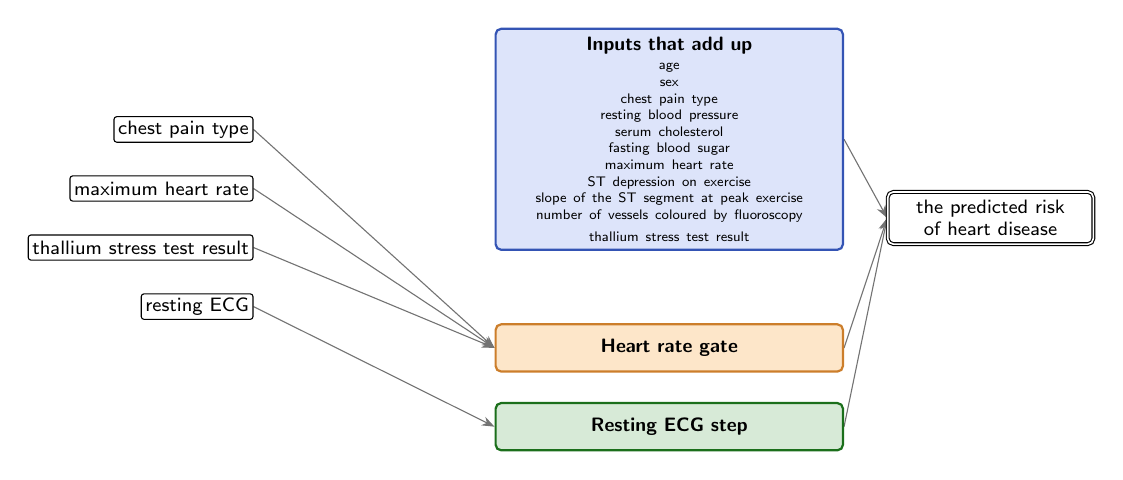
\begin{tikzpicture}[
  font=\sffamily\scriptsize, >={Stealth[length=1.6mm]},
  inp/.style={draw, rounded corners=1pt, fill=white, inner sep=1.5pt, minimum height=3.2mm, anchor=east},
  abox/.style={draw, thick, rounded corners=2pt, align=center, inner sep=3pt, minimum height=6mm, text width=42mm},
  outp/.style={draw, double, rounded corners=2pt, fill=white, align=center, inner sep=3pt, text width=24mm},
  agg/.style={draw=black!55},
]
\node[inp] (i0) at (0,1.125) {chest pain type};
\node[inp] (i1) at (0,0.375) {maximum heart rate};
\node[inp] (i2) at (0,-0.375) {thallium stress test result};
\node[inp] (i3) at (0,-1.125) {resting ECG};
\node[abox, fill=RoyalBlue!18, draw=RoyalBlue!80!black] (b0) at (5.28,1.0) {\textbf{Inputs that add up}\\[1pt]{\tiny age\\ sex\\ chest pain type\\ resting blood pressure\\ serum cholesterol\\ fasting blood sugar\\ maximum heart rate\\ ST depression on exercise\\ slope of the ST segment at peak exercise\\ number of vessels coloured by fluoroscopy\\ thallium stress test result}};
\node[abox, fill=BurntOrange!18, draw=BurntOrange!80!black] (b1) at (5.28,-1.65) {\textbf{Heart rate gate}};
\node[abox, fill=ForestGreen!18, draw=ForestGreen!80!black] (b2) at (5.28,-2.65) {\textbf{Resting ECG step}};
\node[outp] (out) at (9.36,0) {the predicted risk of heart disease};
\begin{scope}[on background layer]
\draw[->, agg] (b0.east) -- (out.west);
\draw[->, agg, thin] (i0.east) -- (b1.west);
\draw[->, agg, thin] (i1.east) -- (b1.west);
\draw[->, agg, thin] (i2.east) -- (b1.west);
\draw[->, agg] (b1.east) -- (out.west);
\draw[->, agg, thin] (i3.east) -- (b2.west);
\draw[->, agg] (b2.east) -- (out.west);
\end{scope}
\end{tikzpicture}}}%
\caption{The model at the level of the summary: one box per part.}
\label{fig:hearts2c2:summary}
\end{figure}
\paragraph{Inputs that add up.} \par\noindent\textit{Lowering the risk.}  These add up independently, and these lower the risk: through this sum alone, compared with no chest pain symptoms, typical angina takes a typical patient's predicted risk from about 32\% to about 2\%, non-anginal chest pain to about 7\% and atypical angina to about 14\%; being a woman lowers it to about 4\% and fasting blood sugar above 120 mg/dL to about 20\%; and a higher maximum heart rate lowers it steadily, from about 37\% at 118 to about 28\% at 175 beats per minute (chest pain type and maximum heart rate also act through the heart rate gate, below).\,{\scriptsize\textcolor{NavyBlue}{[C04, C12, C16, C08, C18, C20]}} \par\noindent\textit{Raising the risk.}  Each extra vessel coloured by fluoroscopy adds about the same, from about 32\% at 0 to about 96\% at 2 vessels, flattening out near the top because the predicted risk cannot go much higher; a flat rather than upsloping ST segment raises it to about 81\%; and ST depression on exercise, cholesterol and resting blood pressure each raise it steadily, from about 25\% at 0 mm to about 55\% at 2.8 mm, from about 22\% at 193 mg/dL to about 50\% at 308 mg/dL, and from about 21\% at 110 mm Hg to about 48\% at 155 mm Hg.\,{\scriptsize\textcolor{NavyBlue}{[C01, C02, C03, C07, C09]}} Through this sum alone a reversible defect on the thallium scan raises it to about 57\% (the thallium scan also acts through the heart rate gate, below); older age raises it steadily but only from about 31\% at 42 to about 32\% at 66 years; and the model ignores chest pain brought on by exercise.\,{\scriptsize\textcolor{NavyBlue}{[C10, C21, C28]}} \par\noindent\textit{Rare results.}  Some rarer results also count (the model has little data on this, n = 15 to 17): a downsloping ST segment raises the risk to about 54\%, and through this sum alone a fixed defect on the thallium scan lowers it to about 12\%.\,{\scriptsize\textcolor{NavyBlue}{[C13, C14]}}
\paragraph{Heart rate gate.} This part reads chest pain type, maximum heart rate and the thallium scan, and acts on 104 of 242 training patients, 24 of whom had heart disease; for the typical patient it acts on, the predicted risk is about 5\% without it and about 2\% with it.\,{\scriptsize\textcolor{NavyBlue}{[C37]}} Across the whole model, non-anginal chest pain lowers the predicted risk, and even more so without a fixed defect on the thallium scan: from about 32\% to about 3\% then, against about 12\% to about 2\% with one (the model has little data on this, n = 15).\,{\scriptsize\textcolor{NavyBlue}{[C33]}} Across the whole model, a higher maximum heart rate lowers the risk, and even more so with non-anginal chest pain, where it falls steadily from about 7\% at 118 to about 2\% at 175 beats per minute, flattening out near the bottom because the predicted risk cannot go much lower; for other chest pain types it falls from about 37\% to about 26\%.\,{\scriptsize\textcolor{NavyBlue}{[C35]}} Through this part alone, for most patients a higher maximum heart rate does nothing until about 168 beats per minute, then lowers the risk steadily, but for patients with non-anginal chest pain it lowers it steadily all along: for a typical patient from about 32\% at 118 to about 29\% at 175 beats per minute (the model has little data on this, n = 14).\,{\scriptsize\textcolor{NavyBlue}{[C31, C36]}}
\paragraph{Resting ECG step.} This part reads only the resting ECG: signs of left ventricular hypertrophy take a typical patient's predicted risk from about 32\% to about 31\%, and switching the part off changes any prediction by at most about half a percentage point.\,{\scriptsize\textcolor{NavyBlue}{[C39, C41]}}
\paragraph{The whole network.} Figure~\ref{fig:hearts2c2:overview} (next page, landscape) draws every unit and connection of the explained model, nested by part: shaded clusters are the parts of the model and darker boxes the parts inside them; circles are hidden units (h1, h2, \ldots); each cluster's rectangle is its output, and a dashed `sum' stands for an addition the next unit does (drawn, not a unit of the model); the hexagon is the model's output. An input used by several parts is drawn under each of them (same label, dotted outline, the first copy marked with the number of copies): it is the same input, repeated for readability. Not used by the model (input columns with no connection): sugar 120 or less, normal ECG, ST-T abnormal ECG, no exercise pain, exercise pain, downsloping ST, normal thallium, thallium code 4.
\begin{landscape}
\begin{figure}[p]\centering
\resizebox{\linewidth}{!}{%
\definecolor{netup}{HTML}{D95F02}\definecolor{netdown}{HTML}{1B9E77}\definecolor{netmixed}{HTML}{7F7F7F}%
\begin{tikzpicture}[
  font=\sffamily\scriptsize, >={Stealth[length=1.4mm]},
  inp/.style={draw, circle, fill=white, minimum size=3.2mm, inner sep=0pt},
  hid/.style={draw, circle, fill=white, minimum size=5.2mm, inner sep=0.5pt, font=\sffamily\tiny},
  exitbox/.style={draw, thick, rectangle, fill=white, align=center, text width=17mm, minimum height=5mm, inner sep=1.5pt, font=\sffamily\tiny},
  sumbox/.style={draw, thick, dashed, rectangle, fill=white, align=center, text width=17mm, minimum height=5mm, inner sep=1.5pt, font=\sffamily\tiny},
  outp/.style={draw, thick, regular polygon, regular polygon sides=6, fill=white, minimum size=10mm, inner sep=0pt, font=\sffamily\tiny, align=center},
  stub/.style={draw, dashed, rounded corners=2pt, fill=white, align=center, inner sep=2pt, font=\sffamily\tiny, text width=15mm},
  inlab/.style={font=\sffamily\tiny, align=center, text width=15mm, inner sep=1pt, fill=white, fill opacity=0.8, text opacity=1},
  wpos/.style={draw=NavyBlue}, wneg/.style={draw=BrickRed}, wagg/.style={draw=black!45, line width=1.2pt},
  wmix/.style={draw=Plum},
]
\node[outp] (n0) at (11.34,6.15) {heart disease};
\node[hid] (n2472) at (15.94,3.25) {h1};
\node[hid] (n2942) at (15.94,1.9) {h2};
\node[exitbox] (n3607) at (21.78,1.9) {Resting ECG step $\downarrow$};
\node[exitbox] (n3842) at (15.94,4.6) {Heart rate gate $\downarrow$};
\node[sumbox] (nxxsumxx) at (5.85,1.9) {sum: Inputs that add up};
\node[inp, draw=netup, very thick] (ninxxagexxadditive) at (0.9,-2.1) {};
\path (ninxxagexxadditive.south) node[inlab, anchor=north] (labninxxagexxadditive) {age $\uparrow$};
\node[inp, draw=netdown, very thick] (ninxxsexx0xxadditive) at (3.6,-1.05) {};
\path (ninxxsexx0xxadditive.south) node[inlab, anchor=north] (labninxxsexx0xxadditive) {female $\downarrow$};
\node[inp, draw=netup, very thick] (ninxxsexx1xxadditive) at (5.4,-1.05) {};
\path (ninxxsexx1xxadditive.south) node[inlab, anchor=north] (labninxxsexx1xxadditive) {male $\uparrow$};
\node[inp, draw=netdown, very thick] (ninxxcpx1xxadditive) at (9.0,-1.05) {};
\path (ninxxcpx1xxadditive.south) node[inlab, anchor=north] (labninxxcpx1xxadditive) {typical angina $\downarrow$};
\node[inp, draw=netdown, very thick] (ninxxcpx2xxadditive) at (1.8,-1.05) {};
\path (ninxxcpx2xxadditive.south) node[inlab, anchor=north] (labninxxcpx2xxadditive) {atypical angina $\downarrow$};
\node[inp, draw=netup, very thick] (ninxxcpx4xxadditive) at (6.3,-2.1) {};
\path (ninxxcpx4xxadditive.south) node[inlab, anchor=north] (labninxxcpx4xxadditive) {no chest pain $\uparrow$};
\node[inp, draw=netup, very thick] (ninxxtrestbpsxxadditive) at (2.7,0.0) {};
\path (ninxxtrestbpsxxadditive.south) node[inlab, anchor=north] (labninxxtrestbpsxxadditive) {blood pressure $\uparrow$};
\node[inp, draw=netup, very thick] (ninxxcholxxadditive) at (2.7,-2.1) {};
\path (ninxxcholxxadditive.south) node[inlab, anchor=north] (labninxxcholxxadditive) {cholesterol $\uparrow$};
\node[inp, draw=netdown, very thick] (ninxxfbsx1xxadditive) at (8.1,0.0) {};
\path (ninxxfbsx1xxadditive.south) node[inlab, anchor=north] (labninxxfbsx1xxadditive) {sugar above 120 $\downarrow$};
\node[inp, draw=netup, very thick] (ninxxoldpeakxxadditive) at (0.9,0.0) {};
\path (ninxxoldpeakxxadditive.south) node[inlab, anchor=north] (labninxxoldpeakxxadditive) {ST depression $\uparrow$};
\node[inp, draw=netdown, very thick] (ninxxslopex1xxadditive) at (9.9,0.0) {};
\path (ninxxslopex1xxadditive.south) node[inlab, anchor=north] (labninxxslopex1xxadditive) {upsloping ST $\downarrow$};
\node[inp, draw=netup, very thick] (ninxxslopex2xxadditive) at (4.5,-2.1) {};
\path (ninxxslopex2xxadditive.south) node[inlab, anchor=north] (labninxxslopex2xxadditive) {flat ST $\uparrow$};
\node[inp, draw=netup, very thick] (ninxxcaxxadditive) at (10.8,-1.05) {};
\path (ninxxcaxxadditive.south) node[inlab, anchor=north] (labninxxcaxxadditive) {vessels $\uparrow$};
\node[inp, draw=netup, very thick] (ninxxthalx7xxadditive) at (7.2,-1.05) {};
\path (ninxxthalx7xxadditive.south) node[inlab, anchor=north] (labninxxthalx7xxadditive) {reversible defect $\uparrow$};
\node[inp, draw=netdown, very thick] (ninxxcpx3xxannx28) at (17.74,0.0) {};
\path (ninxxcpx3xxannx28.south) node[inlab, anchor=north] (labninxxcpx3xxannx28) {non-anginal pain $\downarrow$};
\node[inp, draw=netdown, very thick] (ninxxrestecgx2xxannx29) at (21.78,0.0) {};
\path (ninxxrestecgx2xxannx29.south) node[inlab, anchor=north] (labninxxrestecgx2xxannx29) {LVH on ECG $\downarrow$};
\node[inp, densely dotted, thick, draw=netdown, very thick] (ninxxthalachxxadditive) at (6.3,0.0) {};
\path (ninxxthalachxxadditive.south) node[inlab, anchor=north] (labninxxthalachxxadditive) {max heart rate ($\times$2) $\downarrow$};
\node[inp, densely dotted, thick, draw=netdown, very thick] (ninxxthalachxxannx28) at (15.94,0.0) {};
\path (ninxxthalachxxannx28.south) node[inlab, anchor=north] (labninxxthalachxxannx28) {max heart rate $\downarrow$};
\node[inp, densely dotted, thick, draw=netdown, very thick] (ninxxthalx6xxadditive) at (4.5,0.0) {};
\path (ninxxthalx6xxadditive.south) node[inlab, anchor=north] (labninxxthalx6xxadditive) {fixed defect ($\times$2) $\downarrow$};
\node[inp, densely dotted, thick, draw=netup, very thick] (ninxxthalx6xxannx28) at (14.14,0.0) {};
\path (ninxxthalx6xxannx28.south) node[inlab, anchor=north] (labninxxthalx6xxannx28) {fixed defect $\uparrow$};
\begin{scope}[on background layer]
\node[fit=(nxxsumxx) , inner sep=8pt, rounded corners=5pt, fill=RoyalBlue!10, draw=RoyalBlue!45] (clu0) {};
\node[fit=(n2472) (n2942) (n3842) , inner sep=8pt, rounded corners=5pt, fill=BurntOrange!10, draw=BurntOrange!45] (clu1) {};
\node[fit=(n3607) , inner sep=8pt, rounded corners=5pt, fill=ForestGreen!10, draw=ForestGreen!45] (clu2) {};
\draw[->, wpos, line width=0.26pt] (ninxxagexxadditive) -- (nxxsumxx);
\draw[->, wneg, line width=0.52pt] (ninxxsexx0xxadditive) -- (nxxsumxx);
\draw[->, wpos, line width=0.37pt] (ninxxsexx1xxadditive) -- (nxxsumxx);
\draw[->, wneg, line width=0.38pt] (ninxxcpx1xxadditive) -- (nxxsumxx);
\draw[->, wpos, line width=0.34pt] (ninxxcpx2xxadditive) -- (nxxsumxx);
\draw[->, wpos, line width=0.55pt] (ninxxcpx4xxadditive) -- (nxxsumxx);
\draw[->, wpos, line width=0.42pt] (ninxxtrestbpsxxadditive) -- (nxxsumxx);
\draw[->, wpos, line width=0.44pt] (ninxxcholxxadditive) -- (nxxsumxx);
\draw[->, wneg, line width=0.33pt] (ninxxfbsx1xxadditive) -- (nxxsumxx);
\draw[->, wpos, line width=0.44pt] (ninxxoldpeakxxadditive) -- (nxxsumxx);
\draw[->, wneg, line width=0.41pt] (ninxxslopex1xxadditive) -- (nxxsumxx);
\draw[->, wpos, line width=0.47pt] (ninxxslopex2xxadditive) -- (nxxsumxx);
\draw[->, wpos, line width=0.87pt] (ninxxcaxxadditive) -- (nxxsumxx);
\draw[->, wpos, line width=0.43pt] (ninxxthalx7xxadditive) -- (nxxsumxx);
\draw[->, wneg, line width=0.26pt] (n3607) -- (n0);
\draw[->, wneg, line width=0.43pt] (n3842) -- (n0);
\draw[->, wpos, line width=0.59pt] (ninxxcpx3xxannx28) -- (n2942);
\draw[->, wpos, line width=0.60pt] (ninxxrestecgx2xxannx29) -- (n3607);
\draw[->, wpos, line width=0.61pt] (n2472) -- (n3842);
\draw[->, wpos, line width=0.61pt] (n2942) -- (n2472);
\draw[->, wneg, line width=0.30pt] (ninxxthalachxxadditive) -- (nxxsumxx);
\draw[->, wpos, line width=0.49pt] (ninxxthalachxxannx28) -- (n2472);
\draw[->, wneg, line width=0.35pt] (ninxxthalx6xxadditive) -- (nxxsumxx);
\draw[->, wneg, line width=0.38pt] (ninxxthalx6xxannx28) -- (n2472);
\draw[->, wagg] (nxxsumxx) -- (n0);
\end{scope}
\node[font=\sffamily\scriptsize\bfseries, text=RoyalBlue!55!black, anchor=south west, inner sep=1pt, fill=white, fill opacity=0.85, text opacity=1] at (clu0.north west) {Inputs that add up};
\node[font=\sffamily\scriptsize\bfseries, text=BurntOrange!55!black, anchor=south west, inner sep=1pt, fill=white, fill opacity=0.85, text opacity=1] at (clu1.north west) {Heart rate gate};
\node[font=\sffamily\scriptsize\bfseries, text=ForestGreen!55!black, anchor=south west, inner sep=1pt, fill=white, fill opacity=0.85, text opacity=1] at (clu2.north west) {Resting ECG step};
\end{tikzpicture}}%
\caption{Every unit and connection of the explained model, nested by part. Blue: positive weight (raises the score); red: negative weight (lowers it); thicker: larger weight. Orange outline and up arrow: raises the final prediction; teal and down arrow: lowers it; grey and double arrow: depends.}
\label{fig:hearts2c2:overview}
\end{figure}
\end{landscape}
\paragraph{Worth checking against what is known.} Worth checking: going from 0 to 2 vessels coloured moves a typical patient's predicted risk from about 32\% to about 96\%.\,{\scriptsize\textcolor{NavyBlue}{[C01]}} Worth checking: patients with typical angina get the lowest predicted risk of all chest pain types, below patients with no chest pain symptoms.\,{\scriptsize\textcolor{NavyBlue}{[C05, C06, C17]}} Worth checking: the model treats fasting blood sugar above 120 mg/dL as lowering the risk of heart disease (for a typical patient from about 32\% to about 20\%).\,{\scriptsize\textcolor{NavyBlue}{[C18]}} Worth checking: the model treats a fixed defect on the thallium scan as lowering the risk (for a typical patient from about 32\% to about 12\%), from only 15 training patients.\,{\scriptsize\textcolor{NavyBlue}{[C15]}} Worth checking: the model ignores whether exercise brings on chest pain.\,{\scriptsize\textcolor{NavyBlue}{[C28]}}
\subsection{The model, read from the top down}
\noindent{\small Each part of the explanation in turn, from the whole model down to the smallest parts: what it does for the prediction (hypothesis), what was checked (evidence), a diagram one level down, and where to read on. The technical record of each part is in ``Technical detail'' at the end.\par}
\subsubsection{The whole model}\label{rd:ann30}
\noindent{\small Figure~\ref{fig:hearts2c2:parts-ann30} shows what feeds this part; Figure~\ref{fig:hearts2c2:units-ann30} its units and every connection into them (dashed boxes: connections from or to other parts, drawn in their own sections).\par}
\begin{figure}[H]\centering
\resizebox{!}{\ifdim\height>0.5\textheight 0.5\textheight\else\height\fi}{%
\resizebox{\ifdim\width>\linewidth\linewidth\else\width\fi}{!}{%
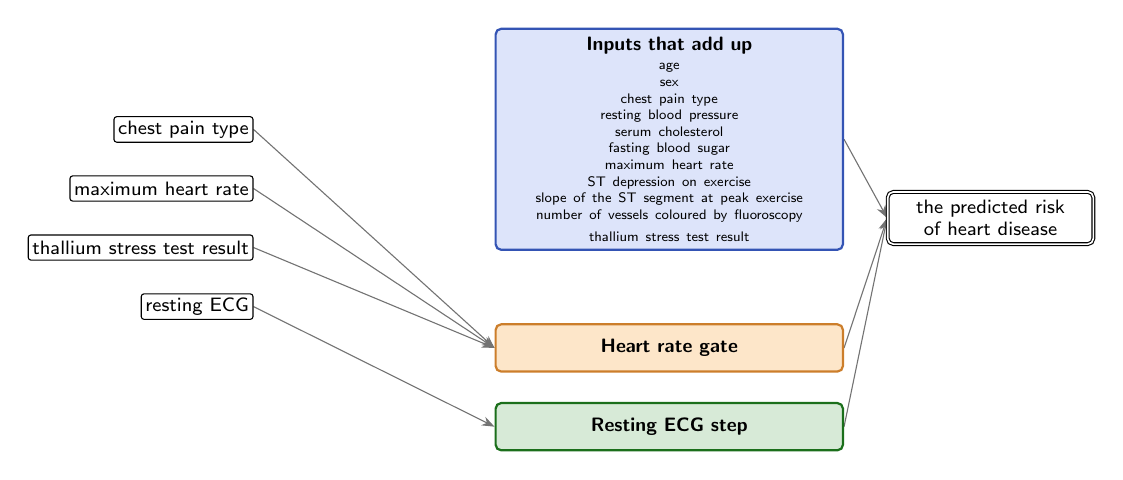
\begin{tikzpicture}[
  font=\sffamily\scriptsize, >={Stealth[length=1.6mm]},
  inp/.style={draw, rounded corners=1pt, fill=white, inner sep=1.5pt, minimum height=3.2mm, anchor=east},
  abox/.style={draw, thick, rounded corners=2pt, align=center, inner sep=3pt, minimum height=6mm, text width=42mm},
  outp/.style={draw, double, rounded corners=2pt, fill=white, align=center, inner sep=3pt, text width=24mm},
  agg/.style={draw=black!55},
]
\node[inp] (i0) at (0,1.125) {chest pain type};
\node[inp] (i1) at (0,0.375) {maximum heart rate};
\node[inp] (i2) at (0,-0.375) {thallium stress test result};
\node[inp] (i3) at (0,-1.125) {resting ECG};
\node[abox, fill=RoyalBlue!18, draw=RoyalBlue!80!black] (b0) at (5.28,1.0) {\textbf{Inputs that add up}\\[1pt]{\tiny age\\ sex\\ chest pain type\\ resting blood pressure\\ serum cholesterol\\ fasting blood sugar\\ maximum heart rate\\ ST depression on exercise\\ slope of the ST segment at peak exercise\\ number of vessels coloured by fluoroscopy\\ thallium stress test result}};
\node[abox, fill=BurntOrange!18, draw=BurntOrange!80!black] (b1) at (5.28,-1.65) {\textbf{Heart rate gate}};
\node[abox, fill=ForestGreen!18, draw=ForestGreen!80!black] (b2) at (5.28,-2.65) {\textbf{Resting ECG step}};
\node[outp] (out) at (9.36,0) {the predicted risk of heart disease};
\begin{scope}[on background layer]
\draw[->, agg] (b0.east) -- (out.west);
\draw[->, agg, thin] (i0.east) -- (b1.west);
\draw[->, agg, thin] (i1.east) -- (b1.west);
\draw[->, agg, thin] (i2.east) -- (b1.west);
\draw[->, agg] (b1.east) -- (out.west);
\draw[->, agg, thin] (i3.east) -- (b2.west);
\draw[->, agg] (b2.east) -- (out.west);
\end{scope}
\end{tikzpicture}}}%
\caption{The whole model: what feeds it, one level down.}
\label{fig:hearts2c2:parts-ann30}
\end{figure}
\begin{figure}[H]\centering
\resizebox{\ifdim\width>\linewidth\linewidth\else\width\fi}{!}{%
\definecolor{netup}{HTML}{D95F02}\definecolor{netdown}{HTML}{1B9E77}\definecolor{netmixed}{HTML}{7F7F7F}%
\begin{tikzpicture}[
  font=\sffamily\scriptsize, >={Stealth[length=1.4mm]},
  inp/.style={draw, circle, fill=white, minimum size=3.2mm, inner sep=0pt},
  hid/.style={draw, circle, fill=white, minimum size=5.2mm, inner sep=0.5pt, font=\sffamily\tiny},
  exitbox/.style={draw, thick, rectangle, fill=white, align=center, text width=17mm, minimum height=5mm, inner sep=1.5pt, font=\sffamily\tiny},
  sumbox/.style={draw, thick, dashed, rectangle, fill=white, align=center, text width=17mm, minimum height=5mm, inner sep=1.5pt, font=\sffamily\tiny},
  outp/.style={draw, thick, regular polygon, regular polygon sides=6, fill=white, minimum size=10mm, inner sep=0pt, font=\sffamily\tiny, align=center},
  stub/.style={draw, dashed, rounded corners=2pt, fill=white, align=center, inner sep=2pt, font=\sffamily\tiny, text width=15mm},
  inlab/.style={font=\sffamily\tiny, align=center, text width=15mm, inner sep=1pt, fill=white, fill opacity=0.8, text opacity=1},
  wpos/.style={draw=NavyBlue}, wneg/.style={draw=BrickRed}, wagg/.style={draw=black!45, line width=1.2pt},
  wmix/.style={draw=Plum},
]
\node[outp] (n0) at (8.42,3.45) {heart disease};
\node[inp, draw=netup, very thick] (ninxxage) at (0.9,-2.1) {};
\path (ninxxage.south) node[inlab, anchor=north] (labninxxage) {age $\uparrow$};
\node[sumbox] (nxxsumxx) at (5.85,1.9) {sum: Inputs that add up};
\node[inp, draw=netdown, very thick] (ninxxsexx0) at (3.6,-1.05) {};
\path (ninxxsexx0.south) node[inlab, anchor=north] (labninxxsexx0) {female $\downarrow$};
\node[inp, draw=netup, very thick] (ninxxsexx1) at (5.4,-1.05) {};
\path (ninxxsexx1.south) node[inlab, anchor=north] (labninxxsexx1) {male $\uparrow$};
\node[inp, draw=netdown, very thick] (ninxxcpx1) at (9.0,-1.05) {};
\path (ninxxcpx1.south) node[inlab, anchor=north] (labninxxcpx1) {typical angina $\downarrow$};
\node[inp, draw=netdown, very thick] (ninxxcpx2) at (1.8,-1.05) {};
\path (ninxxcpx2.south) node[inlab, anchor=north] (labninxxcpx2) {atypical angina $\downarrow$};
\node[inp, draw=netup, very thick] (ninxxcpx4) at (6.3,-2.1) {};
\path (ninxxcpx4.south) node[inlab, anchor=north] (labninxxcpx4) {no chest pain $\uparrow$};
\node[inp, draw=netup, very thick] (ninxxtrestbps) at (2.7,0.0) {};
\path (ninxxtrestbps.south) node[inlab, anchor=north] (labninxxtrestbps) {blood pressure $\uparrow$};
\node[inp, draw=netup, very thick] (ninxxchol) at (2.7,-2.1) {};
\path (ninxxchol.south) node[inlab, anchor=north] (labninxxchol) {cholesterol $\uparrow$};
\node[inp, draw=netdown, very thick] (ninxxfbsx1) at (8.1,0.0) {};
\path (ninxxfbsx1.south) node[inlab, anchor=north] (labninxxfbsx1) {sugar above 120 $\downarrow$};
\node[inp, draw=netup, very thick] (ninxxoldpeak) at (0.9,0.0) {};
\path (ninxxoldpeak.south) node[inlab, anchor=north] (labninxxoldpeak) {ST depression $\uparrow$};
\node[inp, draw=netdown, very thick] (ninxxslopex1) at (9.9,0.0) {};
\path (ninxxslopex1.south) node[inlab, anchor=north] (labninxxslopex1) {upsloping ST $\downarrow$};
\node[inp, draw=netup, very thick] (ninxxslopex2) at (4.5,-2.1) {};
\path (ninxxslopex2.south) node[inlab, anchor=north] (labninxxslopex2) {flat ST $\uparrow$};
\node[inp, draw=netup, very thick] (ninxxca) at (10.8,-1.05) {};
\path (ninxxca.south) node[inlab, anchor=north] (labninxxca) {vessels $\uparrow$};
\node[inp, draw=netup, very thick] (ninxxthalx7) at (7.2,-1.05) {};
\path (ninxxthalx7.south) node[inlab, anchor=north] (labninxxthalx7) {reversible defect $\uparrow$};
\node[stub] (nfromxxRestingxECGxstep) at (15.94,0.0) {from Resting ECG step};
\node[stub] (nfromxxHeartxratexgate) at (14.14,0.0) {from Heart rate gate};
\node[inp, draw=netdown, very thick] (ninxxthalach) at (6.3,0.0) {};
\path (ninxxthalach.south) node[inlab, anchor=north] (labninxxthalach) {max heart rate $\downarrow$};
\node[inp, draw=netdown, very thick] (ninxxthalx6) at (4.5,0.0) {};
\path (ninxxthalx6.south) node[inlab, anchor=north] (labninxxthalx6) {fixed defect $\downarrow$};
\begin{scope}[on background layer]
\node[fit=(nxxsumxx) , inner sep=8pt, rounded corners=5pt, fill=RoyalBlue!10, draw=RoyalBlue!45] (clu0) {};
\draw[->, wpos, line width=0.26pt] (ninxxage) -- (nxxsumxx);
\draw[->, wneg, line width=0.52pt] (ninxxsexx0) -- (nxxsumxx);
\draw[->, wpos, line width=0.37pt] (ninxxsexx1) -- (nxxsumxx);
\draw[->, wneg, line width=0.38pt] (ninxxcpx1) -- (nxxsumxx);
\draw[->, wpos, line width=0.34pt] (ninxxcpx2) -- (nxxsumxx);
\draw[->, wpos, line width=0.55pt] (ninxxcpx4) -- (nxxsumxx);
\draw[->, wpos, line width=0.42pt] (ninxxtrestbps) -- (nxxsumxx);
\draw[->, wpos, line width=0.44pt] (ninxxchol) -- (nxxsumxx);
\draw[->, wneg, line width=0.33pt] (ninxxfbsx1) -- (nxxsumxx);
\draw[->, wpos, line width=0.44pt] (ninxxoldpeak) -- (nxxsumxx);
\draw[->, wneg, line width=0.41pt] (ninxxslopex1) -- (nxxsumxx);
\draw[->, wpos, line width=0.47pt] (ninxxslopex2) -- (nxxsumxx);
\draw[->, wpos, line width=0.87pt] (ninxxca) -- (nxxsumxx);
\draw[->, wpos, line width=0.43pt] (ninxxthalx7) -- (nxxsumxx);
\draw[->, wneg, line width=0.26pt] (nfromxxRestingxECGxstep) -- (n0);
\draw[->, wneg, line width=0.43pt] (nfromxxHeartxratexgate) -- (n0);
\draw[->, wneg, line width=0.30pt] (ninxxthalach) -- (nxxsumxx);
\draw[->, wneg, line width=0.35pt] (ninxxthalx6) -- (nxxsumxx);
\draw[->, wagg] (nxxsumxx) -- (n0);
\end{scope}
\node[font=\sffamily\scriptsize\bfseries, text=RoyalBlue!55!black, anchor=south west, inner sep=1pt, fill=white, fill opacity=0.85, text opacity=1] at (clu0.north west) {Inputs that add up};
\end{tikzpicture}}%
\caption{The whole model: its units and every connection into them. Blue: positive weight (raises the score); red: negative weight (lowers it); thicker: larger weight. Orange outline and up arrow: raises the final prediction; teal and down arrow: lowers it; grey and double arrow: depends.}
\label{fig:hearts2c2:units-ann30}
\end{figure}
\paragraph{Hypothesis.} The model adds up its inputs into one score: the vessels coloured (each extra vessel adding about the same), the ST segment, chest pain type and sex each move the predicted risk on their own, and two parts add to that sum: a heart rate gate that lowers the risk, and a small step for the resting ECG.\,{\scriptsize\textcolor{NavyBlue}{[C29, C01, C02, C05, C08]}}
\paragraph{Evidence.} It is made up of the inputs that feed the score directly and two parts, the heart rate gate and the resting ECG step (each explained below); the score is their sum, which was checked on all 242 training patients.\,{\scriptsize\textcolor{NavyBlue}{[C29]}} Chest pain brought on by exercise feeds nothing, so the model ignores it.\,{\scriptsize\textcolor{NavyBlue}{[C28]}} Across the whole model, compared with no chest pain symptoms, typical angina takes a typical patient's predicted risk from about 32\% to about 2\%, non-anginal chest pain to about 3\% and atypical angina to about 14\%.\,{\scriptsize\textcolor{NavyBlue}{[C05, C06, C17]}} Across the whole model, a higher maximum heart rate lowers the risk, for most patients slowly at first, then faster, but for patients with non-anginal chest pain steadily: from about 37\% at 118 to about 26\% at 175 beats per minute, against about 28\% through the sum alone.\,{\scriptsize\textcolor{NavyBlue}{[C19, C20]}} Across the whole model, a reversible defect on the thallium scan raises it to about 57\%, and a fixed defect lowers it to about 12\% (the model has little data on this, n = 15).\,{\scriptsize\textcolor{NavyBlue}{[C11, C15]}}
\par\noindent{\small Evidence plots: Figure~\ref{fig:hearts2c2:plot-ann30-0}.\par}
\begin{figure}[H]\centering
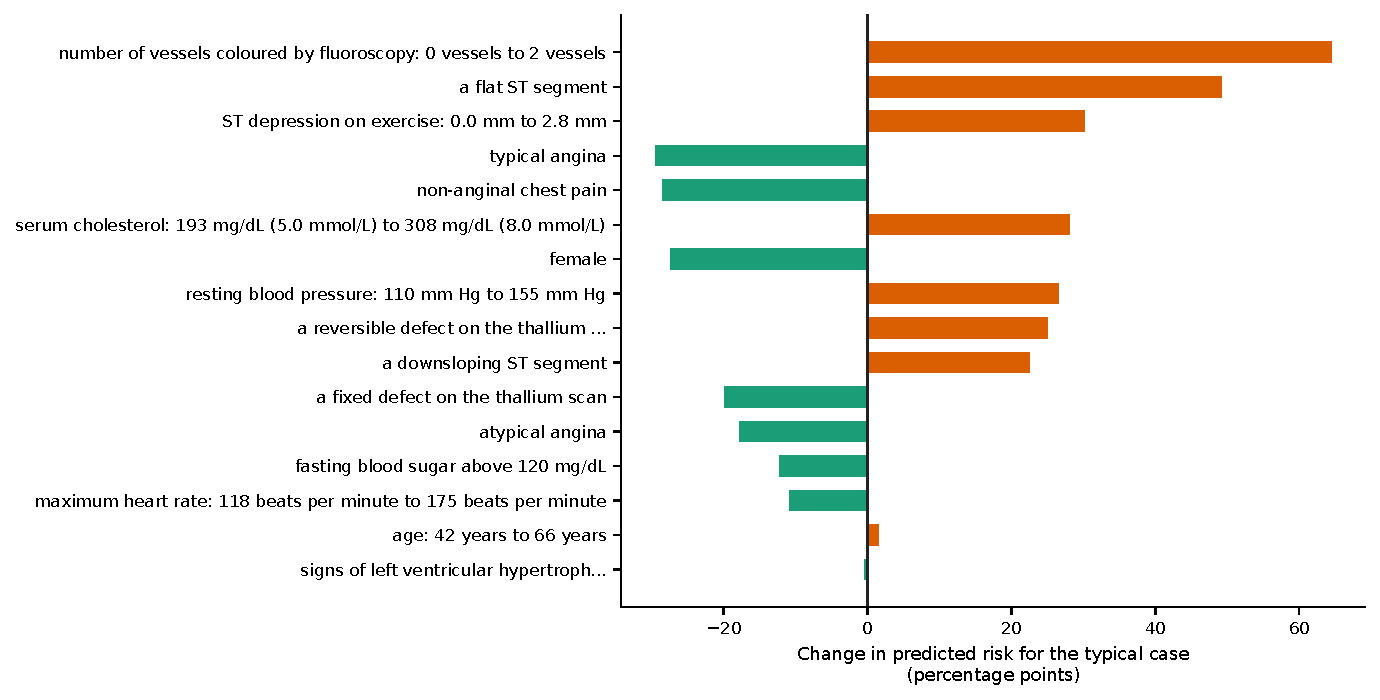
\includegraphics[width=\linewidth,height=0.88\textheight,keepaspectratio]{figures/heart-s2-c2/ann_30-effects.pdf}
\caption{The whole model: Each input's change in the predicted value for the typical case across the whole model, largest first (orange: raises it, teal: lowers it).}
\label{fig:hearts2c2:plot-ann30-0}
\end{figure}
\par\smallskip\noindent{\small \textbf{Dive deeper:} Heart rate gate (\ref{rd:ann28}); Resting ECG step (\ref{rd:ann29}). Technical detail: \ref{tech:ann30}.\par}
\subsubsection{Heart rate gate}\label{rd:ann28}
\noindent{\footnotesize Part of: The whole model (\ref{rd:ann30}).\par}
\noindent{\small Figure~\ref{fig:hearts2c2:parts-ann28} shows what feeds this part; Figure~\ref{fig:hearts2c2:units-ann28} its units and every connection into them (dashed boxes: connections from or to other parts, drawn in their own sections).\par}
\begin{figure}[H]\centering
\resizebox{!}{\ifdim\height>0.5\textheight 0.5\textheight\else\height\fi}{%
\resizebox{\ifdim\width>\linewidth\linewidth\else\width\fi}{!}{%
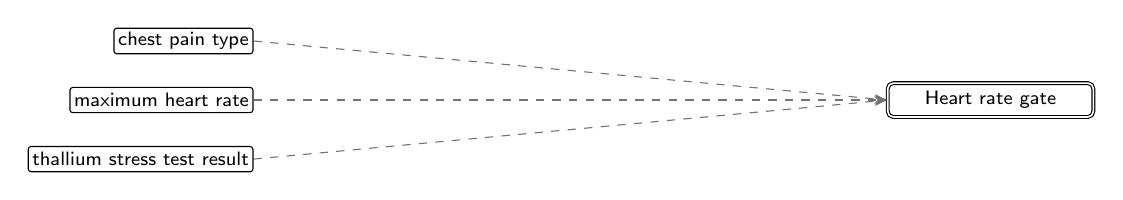
\begin{tikzpicture}[
  font=\sffamily\scriptsize, >={Stealth[length=1.6mm]},
  inp/.style={draw, rounded corners=1pt, fill=white, inner sep=1.5pt, minimum height=3.2mm, anchor=east},
  abox/.style={draw, thick, rounded corners=2pt, align=center, inner sep=3pt, minimum height=6mm, text width=42mm},
  outp/.style={draw, double, rounded corners=2pt, fill=white, align=center, inner sep=3pt, text width=24mm},
  agg/.style={draw=black!55},
]
\node[inp] (i0) at (0,0.75) {chest pain type};
\node[inp] (i1) at (0,-0.0) {maximum heart rate};
\node[inp] (i2) at (0,-0.75) {thallium stress test result};
\node[outp] (out) at (9.36,0) {Heart rate gate};
\begin{scope}[on background layer]
\draw[->, agg, thin, dashed] (i0.east) -- (out.west);
\draw[->, agg, thin, dashed] (i1.east) -- (out.west);
\draw[->, agg, thin, dashed] (i2.east) -- (out.west);
\end{scope}
\end{tikzpicture}}}%
\caption{Heart rate gate: what feeds it, one level down.}
\label{fig:hearts2c2:parts-ann28}
\end{figure}
\begin{figure}[H]\centering
\resizebox{\ifdim\width>\linewidth\linewidth\else\width\fi}{!}{%
\definecolor{netup}{HTML}{D95F02}\definecolor{netdown}{HTML}{1B9E77}\definecolor{netmixed}{HTML}{7F7F7F}%
\begin{tikzpicture}[
  font=\sffamily\scriptsize, >={Stealth[length=1.4mm]},
  inp/.style={draw, circle, fill=white, minimum size=3.2mm, inner sep=0pt},
  hid/.style={draw, circle, fill=white, minimum size=5.2mm, inner sep=0.5pt, font=\sffamily\tiny},
  exitbox/.style={draw, thick, rectangle, fill=white, align=center, text width=17mm, minimum height=5mm, inner sep=1.5pt, font=\sffamily\tiny},
  sumbox/.style={draw, thick, dashed, rectangle, fill=white, align=center, text width=17mm, minimum height=5mm, inner sep=1.5pt, font=\sffamily\tiny},
  outp/.style={draw, thick, regular polygon, regular polygon sides=6, fill=white, minimum size=10mm, inner sep=0pt, font=\sffamily\tiny, align=center},
  stub/.style={draw, dashed, rounded corners=2pt, fill=white, align=center, inner sep=2pt, font=\sffamily\tiny, text width=15mm},
  inlab/.style={font=\sffamily\tiny, align=center, text width=15mm, inner sep=1pt, fill=white, fill opacity=0.8, text opacity=1},
  wpos/.style={draw=NavyBlue}, wneg/.style={draw=BrickRed}, wagg/.style={draw=black!45, line width=1.2pt},
  wmix/.style={draw=Plum},
]
\node[exitbox] (n3842) at (2.7,4.6) {Heart rate gate $\downarrow$};
\node[hid] (n2942) at (2.7,1.9) {h2};
\node[hid] (n2472) at (2.7,3.25) {h1};
\node[inp, draw=netdown, very thick] (ninxxcpx3) at (4.5,0.0) {};
\path (ninxxcpx3.south) node[inlab, anchor=north] (labninxxcpx3) {non-anginal pain $\downarrow$};
\node[inp, draw=netdown, very thick] (ninxxthalach) at (2.7,0.0) {};
\path (ninxxthalach.south) node[inlab, anchor=north] (labninxxthalach) {max heart rate $\downarrow$};
\node[inp, draw=netup, very thick] (ninxxthalx6) at (0.9,0.0) {};
\path (ninxxthalx6.south) node[inlab, anchor=north] (labninxxthalx6) {fixed defect $\uparrow$};
\node[stub] (ntoxxthexmodelxoutput) at (2.7,6.15) {to the model output};
\begin{scope}[on background layer]
\node[fit=(n3842) (n2942) (n2472) , inner sep=8pt, rounded corners=5pt, fill=BurntOrange!10, draw=BurntOrange!45] (clu0) {};
\draw[->, wpos, line width=0.59pt] (ninxxcpx3) -- (n2942);
\draw[->, wpos, line width=0.61pt] (n2472) -- (n3842);
\draw[->, wpos, line width=0.61pt] (n2942) -- (n2472);
\draw[->, wpos, line width=0.49pt] (ninxxthalach) -- (n2472);
\draw[->, wneg, line width=0.38pt] (ninxxthalx6) -- (n2472);
\draw[->, wneg, line width=0.43pt] (n3842) -- (ntoxxthexmodelxoutput);
\end{scope}
\node[font=\sffamily\scriptsize\bfseries, text=BurntOrange!55!black, anchor=south west, inner sep=1pt, fill=white, fill opacity=0.85, text opacity=1] at (clu0.north west) {Heart rate gate};
\end{tikzpicture}}%
\caption{Heart rate gate: its units and every connection into them. Blue: positive weight (raises the score); red: negative weight (lowers it); thicker: larger weight. Orange outline and up arrow: raises the final prediction; teal and down arrow: lowers it; grey and double arrow: depends.}
\label{fig:hearts2c2:units-ann28}
\end{figure}
\paragraph{Hypothesis.} This part lowers the predicted risk for patients with non-anginal chest pain or a high maximum heart rate, unless the thallium scan shows a fixed defect (the model has little data on this, n = 15).\,{\scriptsize\textcolor{NavyBlue}{[C37, C33]}}
\paragraph{Evidence.} It acts on 104 of 242 training patients, 24 of whom had heart disease; for the typical patient it acts on, the predicted risk is about 5\% without it and about 2\% with it.\,{\scriptsize\textcolor{NavyBlue}{[C37]}} Through it, non-anginal chest pain takes a typical patient's predicted risk from about 32\% to about 16\%, and for the typical patient it acts on a fixed defect on the thallium scan raises it from about 2\% to about 4\% (the model has little data on this, n = 15).\,{\scriptsize\textcolor{NavyBlue}{[C30, C32]}} Through it, for most patients a higher maximum heart rate does nothing until about 168 beats per minute, then lowers the risk steadily, but for patients with non-anginal chest pain it lowers it steadily all along: for a typical patient from about 32\% at 118 to about 29\% at 175 beats per minute (the model has little data on this, n = 14).\,{\scriptsize\textcolor{NavyBlue}{[C31, C36]}} Across the whole model, a higher maximum heart rate lowers the risk more without a fixed defect on the thallium scan, for most patients slowly at first, then faster, but for patients with non-anginal chest pain steadily: from about 37\% to about 26\%, against about 14\% to about 10\% with one (the model has little data on this, n = 15).\,{\scriptsize\textcolor{NavyBlue}{[C34]}} Its formula reproduces the part exactly on all 242 training patients.\,{\scriptsize\textcolor{NavyBlue}{[C38]}}
\par\noindent{\small Evidence plots: Figure~\ref{fig:hearts2c2:plot-ann28-0}, Figure~\ref{fig:hearts2c2:plot-ann28-1}, Figure~\ref{fig:hearts2c2:plot-ann28-2}, Figure~\ref{fig:hearts2c2:plot-ann28-3}, Figure~\ref{fig:hearts2c2:plot-ann28-4}.\par}
\par\noindent{\small Figure~\ref{fig:hearts2c2:plot-ann28-3} shows this part's own output, unit h4: it switches on at about 167.7 beats per minute of maximum heart rate, and is zero below.\par}
\begin{figure}[H]\centering
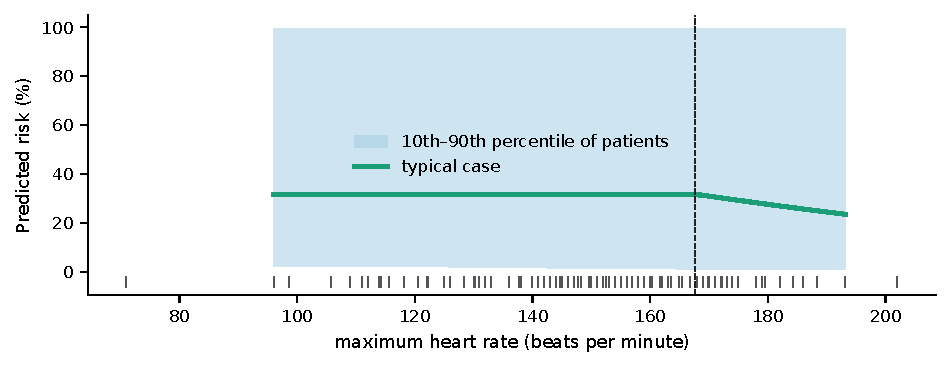
\includegraphics[width=\linewidth,height=0.88\textheight,keepaspectratio]{figures/heart-s2-c2/ann_28-response.pdf}
\caption{Heart rate gate: Response curves through this part: the typical case (bold), the 10th to 90th percentile of individual patients (band), the fold or step point (dashed) with its spread across them (grey), and the observed values (ticks).}
\label{fig:hearts2c2:plot-ann28-0}
\end{figure}
\begin{figure}[H]\centering
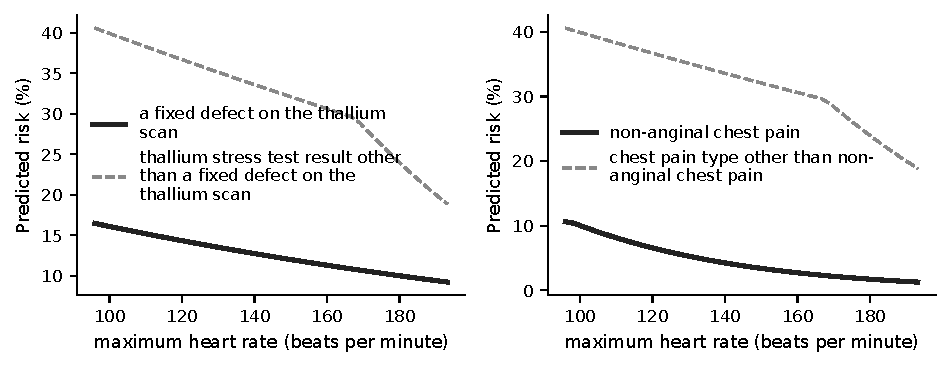
\includegraphics[width=\linewidth,height=0.88\textheight,keepaspectratio]{figures/heart-s2-c2/ann_28-interaction.pdf}
\caption{Heart rate gate: How the effect differs between groups: one curve per group, for the typical case of each group.}
\label{fig:hearts2c2:plot-ann28-1}
\end{figure}
\begin{figure}[H]\centering
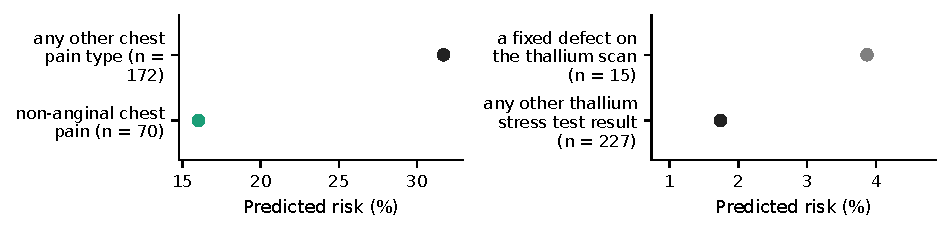
\includegraphics[width=\linewidth,height=0.88\textheight,keepaspectratio]{figures/heart-s2-c2/ann_28-categories-small.pdf}
\caption{Heart rate gate: The predicted value for the typical case at each level, through this part (n = training patients; grey: fewer than 20).}
\label{fig:hearts2c2:plot-ann28-2}
\end{figure}
\begin{figure}[H]\centering
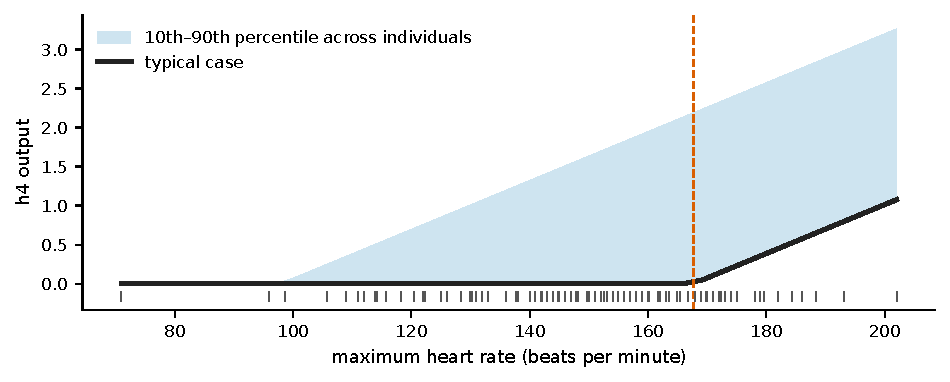
\includegraphics[width=\linewidth,height=0.88\textheight,keepaspectratio]{figures/heart-s2-c2/ann_28-partial-3842.pdf}
\caption{Heart rate gate: This part's own output, unit h4 (the output of 'Heart rate gate'), on its own scale (its activation), with every other input at the typical case; it is active for 104 of 242. Bold: the typical case; band: 10th to 90th percentile across individuals; dashed: where it switches on; ticks: the data.}
\label{fig:hearts2c2:plot-ann28-3}
\end{figure}
\begin{figure}[H]\centering
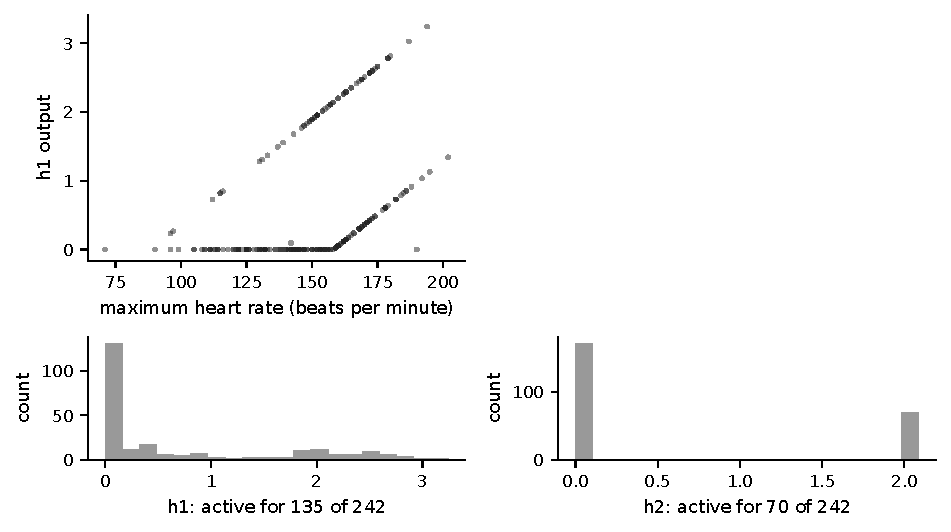
\includegraphics[width=\linewidth,height=0.88\textheight,keepaspectratio]{figures/heart-s2-c2/ann_28-units.pdf}
\caption{Heart rate gate: This part's hidden units: each unit's output against its main numeric input (top) and how often it is active (bottom).}
\label{fig:hearts2c2:plot-ann28-4}
\end{figure}
\par\smallskip\noindent{\small Technical detail: \ref{tech:ann28}.\par}
\subsubsection{Resting ECG step}\label{rd:ann29}
\noindent{\footnotesize Part of: The whole model (\ref{rd:ann30}).\par}
\noindent{\small Figure~\ref{fig:hearts2c2:parts-ann29} shows what feeds this part; Figure~\ref{fig:hearts2c2:units-ann29} its units and every connection into them (dashed boxes: connections from or to other parts, drawn in their own sections).\par}
\begin{figure}[H]\centering
\resizebox{!}{\ifdim\height>0.5\textheight 0.5\textheight\else\height\fi}{%
\resizebox{\ifdim\width>\linewidth\linewidth\else\width\fi}{!}{%
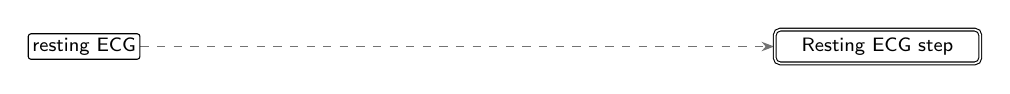
\begin{tikzpicture}[
  font=\sffamily\scriptsize, >={Stealth[length=1.6mm]},
  inp/.style={draw, rounded corners=1pt, fill=white, inner sep=1.5pt, minimum height=3.2mm, anchor=east},
  abox/.style={draw, thick, rounded corners=2pt, align=center, inner sep=3pt, minimum height=6mm, text width=42mm},
  outp/.style={draw, double, rounded corners=2pt, fill=white, align=center, inner sep=3pt, text width=24mm},
  agg/.style={draw=black!55},
]
\node[inp] (i0) at (0,-0.0) {resting ECG};
\node[outp] (out) at (9.36,0) {Resting ECG step};
\begin{scope}[on background layer]
\draw[->, agg, thin, dashed] (i0.east) -- (out.west);
\end{scope}
\end{tikzpicture}}}%
\caption{Resting ECG step: what feeds it, one level down.}
\label{fig:hearts2c2:parts-ann29}
\end{figure}
\begin{figure}[H]\centering
\resizebox{\ifdim\width>\linewidth\linewidth\else\width\fi}{!}{%
\definecolor{netup}{HTML}{D95F02}\definecolor{netdown}{HTML}{1B9E77}\definecolor{netmixed}{HTML}{7F7F7F}%
\begin{tikzpicture}[
  font=\sffamily\scriptsize, >={Stealth[length=1.4mm]},
  inp/.style={draw, circle, fill=white, minimum size=3.2mm, inner sep=0pt},
  hid/.style={draw, circle, fill=white, minimum size=5.2mm, inner sep=0.5pt, font=\sffamily\tiny},
  exitbox/.style={draw, thick, rectangle, fill=white, align=center, text width=17mm, minimum height=5mm, inner sep=1.5pt, font=\sffamily\tiny},
  sumbox/.style={draw, thick, dashed, rectangle, fill=white, align=center, text width=17mm, minimum height=5mm, inner sep=1.5pt, font=\sffamily\tiny},
  outp/.style={draw, thick, regular polygon, regular polygon sides=6, fill=white, minimum size=10mm, inner sep=0pt, font=\sffamily\tiny, align=center},
  stub/.style={draw, dashed, rounded corners=2pt, fill=white, align=center, inner sep=2pt, font=\sffamily\tiny, text width=15mm},
  inlab/.style={font=\sffamily\tiny, align=center, text width=15mm, inner sep=1pt, fill=white, fill opacity=0.8, text opacity=1},
  wpos/.style={draw=NavyBlue}, wneg/.style={draw=BrickRed}, wagg/.style={draw=black!45, line width=1.2pt},
  wmix/.style={draw=Plum},
]
\node[exitbox] (n3607) at (1.6,1.9) {Resting ECG step $\downarrow$};
\node[inp, draw=netdown, very thick] (ninxxrestecgx2) at (1.6,0.0) {};
\path (ninxxrestecgx2.south) node[inlab, anchor=north] (labninxxrestecgx2) {LVH on ECG $\downarrow$};
\node[stub] (ntoxxthexmodelxoutput) at (1.6,3.45) {to the model output};
\begin{scope}[on background layer]
\node[fit=(n3607) , inner sep=8pt, rounded corners=5pt, fill=ForestGreen!10, draw=ForestGreen!45] (clu0) {};
\draw[->, wpos, line width=0.60pt] (ninxxrestecgx2) -- (n3607);
\draw[->, wneg, line width=0.26pt] (n3607) -- (ntoxxthexmodelxoutput);
\end{scope}
\node[font=\sffamily\scriptsize\bfseries, text=ForestGreen!55!black, anchor=south west, inner sep=1pt, fill=white, fill opacity=0.85, text opacity=1] at (clu0.north west) {Resting ECG step};
\end{tikzpicture}}%
\caption{Resting ECG step: its units and every connection into them. Blue: positive weight (raises the score); red: negative weight (lowers it); thicker: larger weight. Orange outline and up arrow: raises the final prediction; teal and down arrow: lowers it; grey and double arrow: depends.}
\label{fig:hearts2c2:units-ann29}
\end{figure}
\paragraph{Hypothesis.} This part barely changes the predictions: signs of left ventricular hypertrophy on the resting ECG take a typical patient's predicted risk from about 32\% to about 31\%.\,{\scriptsize\textcolor{NavyBlue}{[C39, C41]}}
\paragraph{Evidence.} Switching it off changes any training patient's predicted risk by at most about half a percentage point.\,{\scriptsize\textcolor{NavyBlue}{[C41]}} Its formula reproduces the part exactly on all 242 training patients.\,{\scriptsize\textcolor{NavyBlue}{[C42]}}
\par\noindent{\small Evidence plots: Figure~\ref{fig:hearts2c2:plot-ann29-0}, Figure~\ref{fig:hearts2c2:plot-ann29-1}.\par}
\begin{figure}[H]\centering
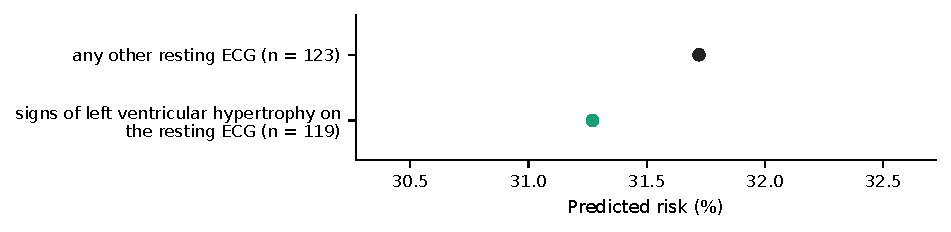
\includegraphics[width=\linewidth,height=0.88\textheight,keepaspectratio]{figures/heart-s2-c2/ann_29-categories-small.pdf}
\caption{Resting ECG step: The predicted value for the typical case at each level, through this part (n = training patients; grey: fewer than 20).}
\label{fig:hearts2c2:plot-ann29-0}
\end{figure}
\begin{figure}[H]\centering
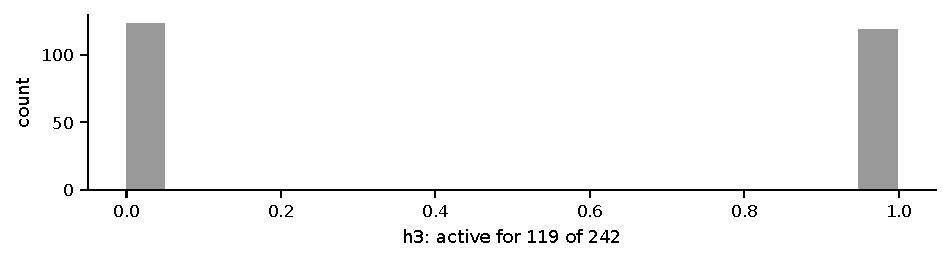
\includegraphics[width=\linewidth,height=0.88\textheight,keepaspectratio]{figures/heart-s2-c2/ann_29-units.pdf}
\caption{Resting ECG step: This part's hidden units: each unit's output against its main numeric input (top) and how often it is active (bottom).}
\label{fig:hearts2c2:plot-ann29-1}
\end{figure}
\par\smallskip\noindent{\small Technical detail: \ref{tech:ann29}.\par}
\subsection{Not supported by the model}
\begin{itemize}\setlength\itemsep{0pt}\small
\item C40: subgroup claim about resting ECG in part ann\_\allowbreak{}29: not supported by the model (its effect is negligible).
\end{itemize}
\clearpage\section*{Technical detail: heart-s2-c2}
\addcontentsline{toc}{section}{Technical detail: heart-s2-c2}
\noindent{\small The record behind each part: the original hypothesis, the closed form, and every claim with its estimate (log-odds and odds ratio), range across patients, n and test check.\par}
\renewcommand{\thesubsection}{T.\arabic{subsection}}\setcounter{subsection}{0}
\subsection{The whole model}\label{tech:ann30}
\noindent{\footnotesize Annotation ann\_\allowbreak{}30 (heart\_\allowbreak{}disease\_\allowbreak{}logit). Reads: age, sex, chest pain type, resting blood pressure, serum cholesterol, fasting blood sugar, resting ECG, maximum heart rate reached during the exercise test, exercise-induced angina, ST depression during exercise (compared with rest), slope of the ST segment at peak exercise, number of major vessels coloured by fluoroscopy, thallium stress test result.\par}
\paragraph{Original hypothesis (unchanged).} Root: heart-disease logit at output 0 (sigmoid). Essentially logistic regression: 16 direct edges (ca +1.78, cp:4 +0.87, sex:0 -0.77, slope:2 +0.63, oldpeak +0.56, chol +0.54, thal:7 +0.50, trestbps +0.49, slope:1 -0.47, cp:1 -0.37, sex:1 +0.34, thal:6 -0.30, cp:2 +0.26, fbs:1 -0.22, thalach -0.15, age +0.03) carry logit SD 3.66 and train AUC 0.9343 alone (L2 logistic regression on all 26 inputs: 0.9355). The two children are added to the logit: heart\_\allowbreak{}rate\_\allowbreak{}nonanginal\_\allowbreak{}gate (x -0.519; +0.006 AUC, the only consequential nonlinearity) and restecg2\_\allowbreak{}relay (x -0.021, negligible). Eight inputs are unconnected, zero effect: thal:3, thal:4, slope:3, exang:0, exang:1, restecg:0, restecg:1, fbs:0 (exercise angina is ignored). Evidence (train, n=242): composed closed form; sensitivity and mean $|$SHAP$|$ both rank ca first (0.16), then cp:4, sex:0, slope:2; full-model train AUC 0.9403, accuracy 0.897.
\paragraph{Closed form.} Read through its parts (their formulas are in their own sections).
\paragraph{Split inputs.} To annotate the parts, the explanation split these inputs into copies (a refactoring step that does not change what the model computes); the diagrams draw each input once: fixed defect (2 copies); max heart rate (2 copies).
\paragraph{Evidence table} (next page, landscape).
\begin{landscape}
{\scriptsize\setlength{\tabcolsep}{3pt}\renewcommand{\arraystretch}{1.15}
\rowcolors{2}{black!6}{white}
\begin{longtable}{@{}l>{\raggedright\arraybackslash}p{0.36\linewidth}>{\raggedright\arraybackslash}p{0.14\linewidth}rrr>{\raggedright\arraybackslash}p{0.06\linewidth}>{\raggedright\arraybackslash}p{0.17\linewidth}c@{}}
\toprule\rowcolor{white}
ID & What is checked & Risk, typical patient & Log-odds & OR & Range (p10--p90) & n & Test check & OK \\
\midrule\endfirsthead
\toprule\rowcolor{white}
ID & What is checked & Risk, typical patient & Log-odds & OR & Range (p10--p90) & n & Test check & OK \\
\midrule\endhead
\bottomrule\endfoot
C01 & direction: number of vessels coloured by fluoroscopy: 0 vessels to 2 vessels (whole model) \newline{\itshape shape: steady (equal steps); 100\% of patients same; verified; risk saturates near 100\%} & 32\% to 96\% & 3.99 & 54.0 & 3.99 to 3.99 & 242 & unclear; AUC gain 0.037 [-0.038, 0.119] & \textcolor{OliveGreen}{yes} \\
C02 & direction: slope of the ST segment at peak exercise: an upsloping ST segment to a flat ST segment (whole model) \newline{\itshape shape: categorical; highest to lowest: a flat ST segment, a downsloping ST segment, an upsloping ST segment} & 32\% to 81\% & 2.21 & 9.14 & 2.21 to 2.21 & 115, 110 & disagrees; AUC gain -0.004 [-0.044, 0.034] & \textcolor{OliveGreen}{yes} \\
C03 & direction: ST depression on exercise: 0.0 mm to 2.8 mm (whole model) \newline{\itshape shape: steady; 100\% of patients same; verified} & 25\% to 55\% & 1.31 & 3.72 & 1.31 to 1.31 & 242 & unclear; AUC gain 0.011 [-0.005, 0.034] & \textcolor{OliveGreen}{yes} \\
C04 & direction: chest pain type: no chest pain (asymptomatic) to typical angina (direct contribution only, not through any part) \newline{\itshape shape: categorical; highest to lowest: no chest pain (asymptomatic), atypical angina, non-anginal chest pain, typical angina} & 32\% to 2\% & -3.03 & 0.05 & -3.03 to -3.03 & 108, 22 & agrees; AUC gain 0.039 [0.009, 0.076] & \textcolor{OliveGreen}{yes} \\
C05 & direction: chest pain type: no chest pain (asymptomatic) to typical angina (whole model) \newline{\itshape shape: categorical; highest to lowest: no chest pain (asymptomatic), atypical angina, non-anginal chest pain, typical angina} & 32\% to 2\% & -3.03 & 0.05 & -3.03 to -3.03 & 108, 22 & agrees; AUC gain 0.057 [0.017, 0.104] & \textcolor{OliveGreen}{yes} \\
C06 & direction: chest pain type: no chest pain (asymptomatic) to non-anginal chest pain (whole model) \newline{\itshape shape: categorical; highest to lowest: no chest pain (asymptomatic), atypical angina, non-anginal chest pain, typical angina} & 32\% to 3\% & -2.53 & 0.08 & -2.88 to -1.96 & 108, 70 & agrees; AUC gain 0.057 [0.017, 0.104] & \textcolor{OliveGreen}{yes} \\
C07 & direction: serum cholesterol: 193 mg/dL (5.0 mmol/L) to 308 mg/dL (8.0 mmol/L) (whole model) \newline{\itshape shape: steady; 100\% of patients same; verified} & 22\% to 50\% & 1.28 & 3.58 & 1.28 to 1.28 & 242 & disagrees; AUC gain -0.011 [-0.039, 0.012] & \textcolor{OliveGreen}{yes} \\
C08 & direction: sex: male to female (whole model) \newline{\itshape shape: categorical; highest to lowest: male, female} & 32\% to 4\% & -2.34 & 0.10 & -2.34 to -2.34 & 159, 83 & unclear; AUC gain 0.027 [-0.01, 0.074] & \textcolor{OliveGreen}{yes} \\
C09 & direction: resting blood pressure: 110 mm Hg to 155 mm Hg (whole model) \newline{\itshape shape: steady; 100\% of patients same; verified} & 21\% to 48\% & 1.22 & 3.38 & 1.22 to 1.22 & 242 & unclear; AUC gain 0.009 [-0.013, 0.034] & \textcolor{OliveGreen}{yes} \\
C10 & direction: thallium stress test result: thallium stress test result other than a fixed defect on the thallium scan, a reversible defect on the thallium scan to a reversible defect on the thallium scan (direct contribution only, not through any part) \newline{\itshape shape: categorical; highest to lowest: a reversible defect on the thallium scan, thallium stress test result other than a fixed defect on the thallium scan, a reversible defect on the thallium scan, a fixed defect on the thallium scan} & 32\% to 57\% & 1.04 & 2.82 & 1.04 to 1.04 & 137, 90 & unclear; AUC gain 0.018 [-0.012, 0.053] & \textcolor{OliveGreen}{yes} \\
C11 & direction: thallium stress test result: thallium stress test result other than a fixed defect on the thallium scan, a reversible defect on the thallium scan to a reversible defect on the thallium scan (whole model) \newline{\itshape shape: categorical; highest to lowest: a reversible defect on the thallium scan, thallium stress test result other than a fixed defect on the thallium scan, a reversible defect on the thallium scan, a fixed defect on the thallium scan} & 32\% to 57\% & 1.04 & 2.82 & 1.04 to 1.04 & 137, 90 & unclear; AUC gain 0.018 [-0.012, 0.053] & \textcolor{OliveGreen}{yes} \\
C12 & direction: chest pain type: no chest pain (asymptomatic) to non-anginal chest pain (direct contribution only, not through any part) \newline{\itshape shape: categorical; highest to lowest: no chest pain (asymptomatic), atypical angina, non-anginal chest pain, typical angina} & 32\% to 7\% & -1.75 & 0.17 & -1.75 to -1.75 & 108, 70 & agrees; AUC gain 0.039 [0.009, 0.076] & \textcolor{OliveGreen}{yes} \\
C13 & direction: slope of the ST segment at peak exercise: an upsloping ST segment to a downsloping ST segment (whole model) \newline{\itshape shape: categorical; highest to lowest: a flat ST segment, a downsloping ST segment, an upsloping ST segment} & 32\% to 54\% & 0.94 & 2.56 & 0.94 to 0.94 & 115, 17 (small n) & disagrees; AUC gain -0.004 [-0.044, 0.034] & \textcolor{OliveGreen}{yes} \\
C14 & direction: thallium stress test result: thallium stress test result other than a fixed defect on the thallium scan, a reversible defect on the thallium scan to a fixed defect on the thallium scan (direct contribution only, not through any part) \newline{\itshape shape: categorical; highest to lowest: a reversible defect on the thallium scan, thallium stress test result other than a fixed defect on the thallium scan, a reversible defect on the thallium scan, a fixed defect on the thallium scan} & 32\% to 12\% & -1.24 & 0.29 & -1.24 to -1.24 & 137, 15 (small n) & unclear; AUC gain 0.018 [-0.012, 0.053] & \textcolor{OliveGreen}{yes} \\
C15 & direction: thallium stress test result: thallium stress test result other than a fixed defect on the thallium scan, a reversible defect on the thallium scan to a fixed defect on the thallium scan (whole model) \newline{\itshape shape: categorical; highest to lowest: a reversible defect on the thallium scan, thallium stress test result other than a fixed defect on the thallium scan, a reversible defect on the thallium scan, a fixed defect on the thallium scan} & 32\% to 12\% & -1.00 & 0.37 & -1.24 to -0.42 & 137, 15 (small n) & unclear; AUC gain 0.018 [-0.012, 0.053] & \textcolor{OliveGreen}{yes} \\
C16 & direction: chest pain type: no chest pain (asymptomatic) to atypical angina (direct contribution only, not through any part) \newline{\itshape shape: categorical; highest to lowest: no chest pain (asymptomatic), atypical angina, non-anginal chest pain, typical angina} & 32\% to 14\% & -1.05 & 0.35 & -1.05 to -1.05 & 108, 42 & agrees; AUC gain 0.039 [0.009, 0.076] & \textcolor{OliveGreen}{yes} \\
C17 & direction: chest pain type: no chest pain (asymptomatic) to atypical angina (whole model) \newline{\itshape shape: categorical; highest to lowest: no chest pain (asymptomatic), atypical angina, non-anginal chest pain, typical angina} & 32\% to 14\% & -1.05 & 0.35 & -1.05 to -1.05 & 108, 42 & agrees; AUC gain 0.057 [0.017, 0.104] & \textcolor{OliveGreen}{yes} \\
C18 & direction: fasting blood sugar: fasting blood sugar of 120 mg/dL or less to fasting blood sugar above 120 mg/dL (whole model) \newline{\itshape shape: categorical; highest to lowest: fasting blood sugar of 120 mg/dL or less, fasting blood sugar above 120 mg/dL} & 32\% to 20\% & -0.65 & 0.52 & -0.65 to -0.65 & 209, 33 & unclear; AUC gain 0.000 [-0.011, 0.013] & \textcolor{OliveGreen}{yes} \\
C19 & direction: maximum heart rate: 118 beats per minute to 175 beats per minute (whole model) \newline{\itshape shape: accelerating; 67\% of patients same; mixed (but steady for patients with non-anginal chest pain)} & 37\% to 26\% & -0.73 & 0.48 & -1.32 to -0.51 & 242 & agrees; AUC gain 0.014 [0.002, 0.037] & \textcolor{OliveGreen}{yes} \\
C20 & direction: maximum heart rate: 118 beats per minute to 175 beats per minute (direct contribution only, not through any part) \newline{\itshape shape: steady; 100\% of patients same; verified} & 37\% to 28\% & -0.39 & 0.68 & -0.39 to -0.39 & 242 & unclear; AUC gain 0.006 [0.000, 0.020] & \textcolor{OliveGreen}{yes} \\
C21 & direction: age: 42 years to 66 years (whole model) \newline{\itshape shape: steady; 100\% of patients same; verified} & 31\% to 32\% & 0.07 & 1.08 & 0.07 to 0.07 & 242 & disagrees; AUC gain -0.001 [-0.005, 0.000] & \textcolor{OliveGreen}{yes} \\
C22 & direction: resting ECG: resting ECG other than signs of left ventricular hypertrophy on the resting ECG to signs of left ventricular hypertrophy on the resting ECG (whole model) \newline{\itshape shape: categorical; highest to lowest: resting ECG other than signs of left ventricular hypertrophy on the resting ECG, signs of left ventricular hypertrophy on the resting ECG} & 32\% to 31\% & -0.02 & 0.98 & -0.02 to -0.02 & 123, 119 & unclear; AUC gain 0.000 [0.000, 0.000] & \textcolor{OliveGreen}{yes} \\
C23 & magnitude: number of vessels coloured by fluoroscopy: 0 vessels to 2 vessels, typical patient \newline{\itshape shape: steady (equal steps); 100\% of patients same; verified; risk saturates near 100\%} & 32\% to 96\% & 3.99 & 54.0 &  & 242 & unclear; AUC gain 0.037 [-0.038, 0.119] & \textcolor{OliveGreen}{yes} \\
C24 & magnitude: slope of the ST segment at peak exercise: an upsloping ST segment to a flat ST segment, typical patient \newline{\itshape shape: categorical; highest to lowest: a flat ST segment, a downsloping ST segment, an upsloping ST segment} & 32\% to 81\% & 2.21 & 9.14 &  & 115, 110 & disagrees; AUC gain -0.004 [-0.044, 0.034] & \textcolor{OliveGreen}{yes} \\
C25 & magnitude: ST depression on exercise: 0.0 mm to 2.8 mm, typical patient \newline{\itshape shape: steady; 100\% of patients same; verified} & 25\% to 55\% & 1.31 & 3.72 &  & 242 & unclear; AUC gain 0.011 [-0.005, 0.034] & \textcolor{OliveGreen}{yes} \\
C26 & magnitude: chest pain type: no chest pain (asymptomatic) to typical angina, typical patient \newline{\itshape shape: categorical; highest to lowest: no chest pain (asymptomatic), atypical angina, non-anginal chest pain, typical angina} & 32\% to 2\% & -3.03 & 0.05 &  & 108, 22 & agrees; AUC gain 0.057 [0.017, 0.104] & \textcolor{OliveGreen}{yes} \\
C27 & magnitude: serum cholesterol: 193 mg/dL (5.0 mmol/L) to 308 mg/dL (8.0 mmol/L), typical patient \newline{\itshape shape: steady; 100\% of patients same; verified} & 22\% to 50\% & 1.28 & 3.58 &  & 242 & disagrees; AUC gain -0.011 [-0.039, 0.012] & \textcolor{OliveGreen}{yes} \\
C28 & null: model ignores exercise-induced angina (exact rule) &  & 0.00 &  &  & 242 & train only & \textcolor{OliveGreen}{yes} \\
C29 & structure: made of heart\_\allowbreak{}rate\_\allowbreak{}nonanginal\_\allowbreak{}gate,\allowbreak{} restecg2\_\allowbreak{}relay and inputs age, sex, cp, trestbps, chol, fbs, thalach, oldpeak, slope, ca, thal; added &  &  &  &  & 242 & train only & \textcolor{OliveGreen}{yes} \\
\end{longtable}}
\end{landscape}
\subsection{Heart rate gate}\label{tech:ann28}
\noindent{\footnotesize Annotation ann\_\allowbreak{}28 (heart\_\allowbreak{}rate\_\allowbreak{}nonanginal\_\allowbreak{}gate). Reads: chest pain type, maximum heart rate reached during the exercise test, thallium stress test result.\par}
\paragraph{Original hypothesis (unchanged).} Protective heart-rate gate, gated by chest-pain type and thallium. 2942 = ReLU(0.968 cp:3 + 0.571) is a non-anginal-pain indicator (2.09 for the 70 cp:3 patients, 0 otherwise). 3842 = ReLU(1.021*\allowbreak{}ReLU(0.688 thalach - 0.374 thal:6 + 1.028*2942 - 0.347) - 0.295) is read out -0.519 into the logit. The gate opens once max heart rate passes a threshold set by the other two inputs: about -2.3 SD with non-anginal pain (open for 66 of 68), about +0.78 SD for other pain types without a fixed defect (38 of 159), and never with a fixed thallium defect (0 of 15). Once open, each SD of thalach lowers the logit by 0.36 more (total -0.52 vs -0.15 closed), and non-anginal pain lowers it by about 1.1. Evidence (train, n=242): closed form from get\_\allowbreak{}formula; gate open for 104 patients (disease rate 23\% vs 60\% when closed); logit contribution SD 0.45; removing it drops train AUC 0.9403 -$>$ 0.9344, a linear refit on cp:3, thalach, thal:6 recovers 0.9378 (R2 0.87), so most of its value is the gating rather than the linear trend. It is the model's only consequential nonlinearity.
\paragraph{Closed form} {\footnotesize(weights and biases at 3 significant figures; largest difference from the part on the training patients 4.44089e-16).}
{\small\begingroup\allowdisplaybreaks
\begin{align*}
y_{0} &= \operatorname{relu}\bigl(-0.295 + 1.02 \operatorname{relu}\bigl(-0.347 \\
&\qquad + 0.688 x_{thalach\_b} + 1.03 \operatorname{relu}\bigl(0.571 + 0.968 x_{cp:3}\bigr) \\
&\qquad - 0.374 x_{thal:6\_b}\bigr)\bigr)
\end{align*}\endgroup}

\paragraph{Evidence table} (next page, landscape).
\begin{landscape}
{\scriptsize\setlength{\tabcolsep}{3pt}\renewcommand{\arraystretch}{1.15}
\rowcolors{2}{black!6}{white}
\begin{longtable}{@{}l>{\raggedright\arraybackslash}p{0.36\linewidth}>{\raggedright\arraybackslash}p{0.14\linewidth}rrr>{\raggedright\arraybackslash}p{0.06\linewidth}>{\raggedright\arraybackslash}p{0.17\linewidth}c@{}}
\toprule\rowcolor{white}
ID & What is checked & Risk, typical patient & Log-odds & OR & Range (p10--p90) & n & Test check & OK \\
\midrule\endfirsthead
\toprule\rowcolor{white}
ID & What is checked & Risk, typical patient & Log-odds & OR & Range (p10--p90) & n & Test check & OK \\
\midrule\endhead
\bottomrule\endfoot
C30 & direction: chest pain type: chest pain type other than non-anginal chest pain to non-anginal chest pain (through this part) \newline{\itshape shape: categorical; highest to lowest: chest pain type other than non-anginal chest pain, non-anginal chest pain} & 32\% to 16\% & -0.79 & 0.46 & -1.14 to -0.21 & 172, 70 & unclear; AUC gain 0.008 [-0.012, 0.030] & \textcolor{OliveGreen}{yes} \\
C31 & direction: maximum heart rate: 118 beats per minute to 175 beats per minute (through this part) \newline{\itshape shape: hinge at 168 beats per minute; 70\% of patients same; mixed (but steady for patients with non-anginal chest pain); one point with C36 (median fold 168 beats per minute, typical patient 166 beats per minute, 10th-90th percentile 168 beats per minute to 168 beats per minute)} & 32\% to 29\% & -0.34 & 0.71 & -0.93 to -0.12 & 242 & unclear; AUC gain 0.008 [0.000, 0.022] & \textcolor{OliveGreen}{yes} \\
C32 & direction: thallium stress test result: thallium stress test result other than a fixed defect on the thallium scan to a fixed defect on the thallium scan (through this part) \newline{\itshape shape: categorical; highest to lowest: a fixed defect on the thallium scan, thallium stress test result other than a fixed defect on the thallium scan} & 2\% to 4\% (typical patient this part acts on) & 0.24 & 1.27 & 0.00 to 0.82 & 227, 15 (small n) & unclear; AUC gain 0.001 [0.000, 0.006] & \textcolor{OliveGreen}{yes} \\
C33 & interaction: effect of chest pain type (chest pain type other than non-anginal chest pain to non-anginal chest pain) by thallium stress test result: a fixed defect on the thallium scan minus thallium stress test result other than a fixed defect on the thallium scan; stronger in thallium stress test result other than a fixed defect on the thallium scan \newline{\itshape shape: categorical; highest to lowest: chest pain type other than non-anginal chest pain, non-anginal chest pain} & a fixed defect on the thallium scan: 12\% to 2\%; thallium stress test result other than a fixed defect on the thallium scan: 32\% to 3\% & 0.79 & 2.20 &  & 15, 227 (small n) & agrees; AUC gain 0.001 [0.000, 0.006] & \textcolor{OliveGreen}{yes} \\
C34 & interaction: effect of maximum heart rate (118 beats per minute to 175 beats per minute) by thallium stress test result: a fixed defect on the thallium scan minus thallium stress test result other than a fixed defect on the thallium scan; stronger in thallium stress test result other than a fixed defect on the thallium scan \newline{\itshape shape: accelerating; 70\% of patients same; mixed (but steady for patients with non-anginal chest pain)} & a fixed defect on the thallium scan: 14\% to 10\%; thallium stress test result other than a fixed defect on the thallium scan: 37\% to 26\% & 0.30 & 1.35 &  & 15, 227 (small n) & agrees; AUC gain 0.001 [0.000, 0.006] & \textcolor{OliveGreen}{yes} \\
C35 & interaction: effect of maximum heart rate (118 beats per minute to 175 beats per minute) by chest pain type: non-anginal chest pain minus chest pain type other than non-anginal chest pain; stronger in non-anginal chest pain \newline{\itshape shape: steady; 97\% of patients same; verified; risk saturates near 0\%} & non-anginal chest pain: 7\% to 2\%; chest pain type other than non-anginal chest pain: 37\% to 26\% & -0.80 & 0.45 &  & 70, 172 & agrees; AUC gain 0.008 [-0.012, 0.030] & \textcolor{OliveGreen}{yes} \\
C36 & threshold: maximum heart rate: fold at about 168 beats per minute (starts) for patients with no chest pain symptoms (asymptomatic) \newline{\itshape shape: hinge at 168 beats per minute; 100\% of patients same; verified; risk saturates near 100\%; one point with C36 (median fold 168 beats per minute, typical patient 166 beats per minute, 10th-90th percentile 168 beats per minute to 168 beats per minute)} & 99\% to 99\% (typical patient with a fold (patients with no chest pain symptoms (asymptomatic))) & -0.23 & 0.79 & -0.23 to -0.23 & 99, 14 (small n) & unclear; AUC gain 0.008 [0.000, 0.022] & \textcolor{OliveGreen}{yes} \\
C37 & subgroup: who this part acts on: 104 of 242 patients & 5\% to 2\% (typical patient this part acts on (risk without the part, then with it)) & -0.67 & 0.51 & -1.22 to -0.05 & 104, 138 & unclear; AUC gain 0.018 [0.000, 0.044] & \textcolor{OliveGreen}{yes} \\
C38 & structure: its formula reproduces it on 242 training patients (largest difference 4.44089e-16) &  & 4e-16 &  &  & 242 & train only & \textcolor{OliveGreen}{yes} \\
\end{longtable}}
\end{landscape}
\subsection{Resting ECG step}\label{tech:ann29}
\noindent{\footnotesize Annotation ann\_\allowbreak{}29 (restecg2\_\allowbreak{}relay). Reads: resting ECG.\par}
\paragraph{Original hypothesis (unchanged).} restecg:2 relay: 3607 = ReLU(0.997 restecg:2 - 0.016) is 0.998 for the 119 patients with left ventricular hypertrophy on the resting ECG and 0 for the other 123, i.e. exactly affine in the binary input on the data. Read out -0.021, it lowers the logit by 0.02 for LVH: negligible. Evidence (train, n=242): closed form; entry-exit correlation 1.0; logit SD 0.01; removing it changes train AUC 0.9403 -$>$ 0.9401.
\paragraph{Closed form} {\footnotesize(weights and biases at 3 significant figures; largest difference from the part on the training patients 0.0).}
{\small\begingroup\allowdisplaybreaks
\begin{align*}
y_{0} &= \operatorname{relu}\bigl(-0.016 + 0.997 x_{restecg:2}\bigr)
\end{align*}\endgroup}

\paragraph{Evidence table} (next page, landscape).
\begin{landscape}
{\scriptsize\setlength{\tabcolsep}{3pt}\renewcommand{\arraystretch}{1.15}
\rowcolors{2}{black!6}{white}
\begin{longtable}{@{}l>{\raggedright\arraybackslash}p{0.36\linewidth}>{\raggedright\arraybackslash}p{0.14\linewidth}rrr>{\raggedright\arraybackslash}p{0.06\linewidth}>{\raggedright\arraybackslash}p{0.17\linewidth}c@{}}
\toprule\rowcolor{white}
ID & What is checked & Risk, typical patient & Log-odds & OR & Range (p10--p90) & n & Test check & OK \\
\midrule\endfirsthead
\toprule\rowcolor{white}
ID & What is checked & Risk, typical patient & Log-odds & OR & Range (p10--p90) & n & Test check & OK \\
\midrule\endhead
\bottomrule\endfoot
C39 & direction: resting ECG: resting ECG other than signs of left ventricular hypertrophy on the resting ECG to signs of left ventricular hypertrophy on the resting ECG (through this part) \newline{\itshape shape: categorical; highest to lowest: resting ECG other than signs of left ventricular hypertrophy on the resting ECG, signs of left ventricular hypertrophy on the resting ECG} & 32\% to 31\% & -0.02 & 0.98 & -0.02 to -0.02 & 123, 119 & unclear; AUC gain 0.000 [0.000, 0.000] & \textcolor{OliveGreen}{yes} \\
C40 & subgroup: who this part acts on: 119 of 242 patients & 85\% to 84\% (typical patient this part acts on (risk without the part, then with it)) & -0.02 & 0.98 & -0.02 to -0.02 & 119, 123 & unclear; AUC gain 0.000 [0.000, 0.000] & \textcolor{BrickRed}{no} \\
C41 & null: this part barely changes predictions (switched off) &  & 0.005 &  &  & 242 & train only & \textcolor{OliveGreen}{yes} \\
C42 & structure: its formula reproduces it on 242 training patients (largest difference 0.0) &  & 0.00 &  &  & 242 & train only & \textcolor{OliveGreen}{yes} \\
\end{longtable}}
\end{landscape}
\subsection*{The network before any explanation}\addcontentsline{toc}{subsection}{The network before any explanation} Figure~\ref{fig:hearts2c2:raw} (next page, landscape) is the trained network as it is, with no parts, no splits and no inserted units: inputs at the bottom, hidden units by depth, the output at the top, every connection drawn, every input column its own node (one-hot levels included).
\begin{landscape}
\begin{figure}[p]\centering
\resizebox{\linewidth}{!}{%
\definecolor{netup}{HTML}{D95F02}\definecolor{netdown}{HTML}{1B9E77}\definecolor{netmixed}{HTML}{7F7F7F}%
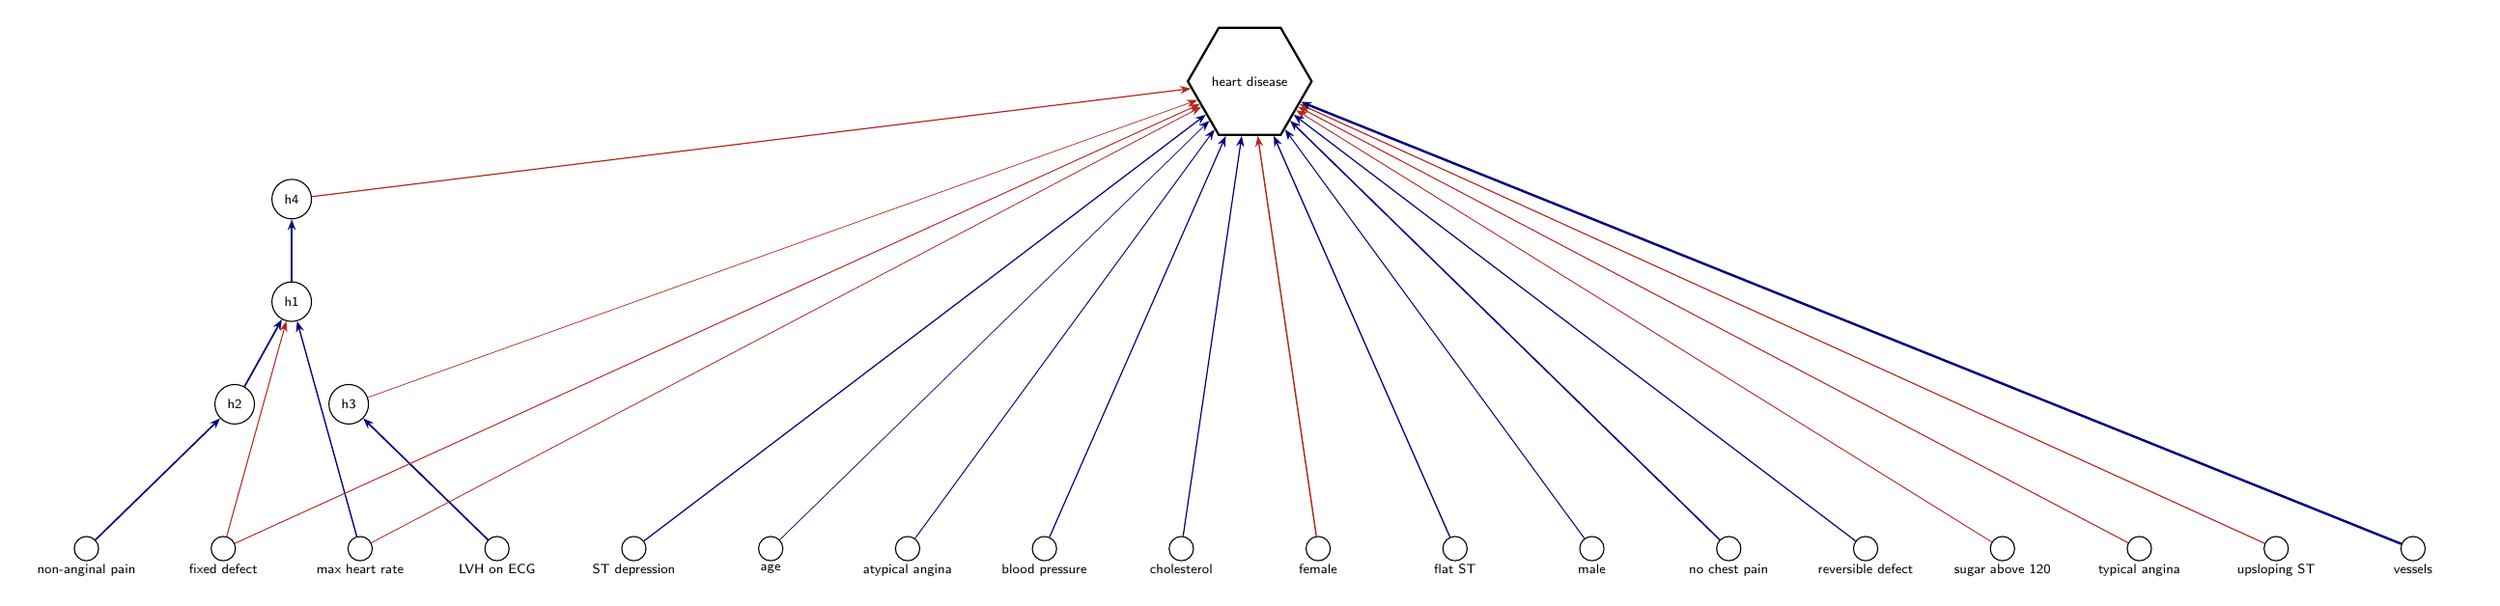
\begin{tikzpicture}[
  font=\sffamily\scriptsize, >={Stealth[length=1.4mm]},
  inp/.style={draw, circle, fill=white, minimum size=3.2mm, inner sep=0pt},
  hid/.style={draw, circle, fill=white, minimum size=5.2mm, inner sep=0.5pt, font=\sffamily\tiny},
  exitbox/.style={draw, thick, rectangle, fill=white, align=center, text width=17mm, minimum height=5mm, inner sep=1.5pt, font=\sffamily\tiny},
  sumbox/.style={draw, thick, dashed, rectangle, fill=white, align=center, text width=17mm, minimum height=5mm, inner sep=1.5pt, font=\sffamily\tiny},
  outp/.style={draw, thick, regular polygon, regular polygon sides=6, fill=white, minimum size=10mm, inner sep=0pt, font=\sffamily\tiny, align=center},
  stub/.style={draw, dashed, rounded corners=2pt, fill=white, align=center, inner sep=2pt, font=\sffamily\tiny, text width=15mm},
  inlab/.style={font=\sffamily\tiny, align=center, text width=15mm, inner sep=1pt, fill=white, fill opacity=0.8, text opacity=1},
  wpos/.style={draw=NavyBlue}, wneg/.style={draw=BrickRed}, wagg/.style={draw=black!45, line width=1.2pt},
  wmix/.style={draw=Plum},
]
\node[inp] (ninxxage) at (9.0,0.0) {};
\path (ninxxage.south) node[inlab, anchor=north] (labninxxage) {age};
\node[inp] (ninxxfbsx1) at (25.2,0.0) {};
\path (ninxxfbsx1.south) node[inlab, anchor=north] (labninxxfbsx1) {sugar above 120};
\node[inp] (ninxxrestecgx2) at (5.4,0.0) {};
\path (ninxxrestecgx2.south) node[inlab, anchor=north] (labninxxrestecgx2) {LVH on ECG};
\node[inp] (ninxxthalach) at (3.6,0.0) {};
\path (ninxxthalach.south) node[inlab, anchor=north] (labninxxthalach) {max heart rate};
\node[inp] (ninxxoldpeak) at (7.2,0.0) {};
\path (ninxxoldpeak.south) node[inlab, anchor=north] (labninxxoldpeak) {ST depression};
\node[inp] (ninxxslopex1) at (28.8,0.0) {};
\path (ninxxslopex1.south) node[inlab, anchor=north] (labninxxslopex1) {upsloping ST};
\node[inp] (ninxxsexx0) at (16.2,0.0) {};
\path (ninxxsexx0.south) node[inlab, anchor=north] (labninxxsexx0) {female};
\node[inp] (ninxxslopex2) at (18.0,0.0) {};
\path (ninxxslopex2.south) node[inlab, anchor=north] (labninxxslopex2) {flat ST};
\node[inp] (ninxxca) at (30.6,0.0) {};
\path (ninxxca.south) node[inlab, anchor=north] (labninxxca) {vessels};
\node[inp] (ninxxthalx6) at (1.8,0.0) {};
\path (ninxxthalx6.south) node[inlab, anchor=north] (labninxxthalx6) {fixed defect};
\node[inp] (ninxxthalx7) at (23.4,0.0) {};
\path (ninxxthalx7.south) node[inlab, anchor=north] (labninxxthalx7) {reversible defect};
\node[inp] (ninxxsexx1) at (19.8,0.0) {};
\path (ninxxsexx1.south) node[inlab, anchor=north] (labninxxsexx1) {male};
\node[inp] (ninxxcpx1) at (27.0,0.0) {};
\path (ninxxcpx1.south) node[inlab, anchor=north] (labninxxcpx1) {typical angina};
\node[inp] (ninxxcpx2) at (10.8,0.0) {};
\path (ninxxcpx2.south) node[inlab, anchor=north] (labninxxcpx2) {atypical angina};
\node[inp] (ninxxcpx3) at (0.0,0.0) {};
\path (ninxxcpx3.south) node[inlab, anchor=north] (labninxxcpx3) {non-anginal pain};
\node[inp] (ninxxcpx4) at (21.6,0.0) {};
\path (ninxxcpx4.south) node[inlab, anchor=north] (labninxxcpx4) {no chest pain};
\node[inp] (ninxxtrestbps) at (12.6,0.0) {};
\path (ninxxtrestbps.south) node[inlab, anchor=north] (labninxxtrestbps) {blood pressure};
\node[inp] (ninxxchol) at (14.4,0.0) {};
\path (ninxxchol.south) node[inlab, anchor=north] (labninxxchol) {cholesterol};
\node[outp] (n0) at (15.3,6.15) {heart disease};
\node[hid] (n2472) at (2.7,3.25) {h1};
\node[hid] (n2942) at (1.95,1.9) {h2};
\node[hid] (n3607) at (3.45,1.9) {h3};
\node[hid] (n3842) at (2.7,4.6) {h4};
\begin{scope}[on background layer]
\draw[->, wpos, line width=0.26pt] (ninxxage) -- (n0);
\draw[->, wneg, line width=0.33pt] (ninxxfbsx1) -- (n0);
\draw[->, wpos, line width=0.60pt] (ninxxrestecgx2) -- (n3607);
\draw[->, wneg, line width=0.30pt] (ninxxthalach) -- (n0);
\draw[->, wpos, line width=0.49pt] (ninxxthalach) -- (n2472);
\draw[->, wpos, line width=0.44pt] (ninxxoldpeak) -- (n0);
\draw[->, wneg, line width=0.41pt] (ninxxslopex1) -- (n0);
\draw[->, wneg, line width=0.52pt] (ninxxsexx0) -- (n0);
\draw[->, wpos, line width=0.47pt] (ninxxslopex2) -- (n0);
\draw[->, wpos, line width=0.87pt] (ninxxca) -- (n0);
\draw[->, wneg, line width=0.35pt] (ninxxthalx6) -- (n0);
\draw[->, wneg, line width=0.38pt] (ninxxthalx6) -- (n2472);
\draw[->, wpos, line width=0.43pt] (ninxxthalx7) -- (n0);
\draw[->, wpos, line width=0.37pt] (ninxxsexx1) -- (n0);
\draw[->, wneg, line width=0.38pt] (ninxxcpx1) -- (n0);
\draw[->, wpos, line width=0.34pt] (ninxxcpx2) -- (n0);
\draw[->, wpos, line width=0.59pt] (ninxxcpx3) -- (n2942);
\draw[->, wpos, line width=0.55pt] (ninxxcpx4) -- (n0);
\draw[->, wpos, line width=0.42pt] (ninxxtrestbps) -- (n0);
\draw[->, wpos, line width=0.44pt] (ninxxchol) -- (n0);
\draw[->, wpos, line width=0.61pt] (n2472) -- (n3842);
\draw[->, wpos, line width=0.61pt] (n2942) -- (n2472);
\draw[->, wneg, line width=0.26pt] (n3607) -- (n0);
\draw[->, wneg, line width=0.43pt] (n3842) -- (n0);
\end{scope}
\end{tikzpicture}}%
\caption{The network as trained, before any explanation, in full. Blue: positive weight (raises the score); red: negative weight (lowers it); thicker: larger weight. Orange outline and up arrow: raises the final prediction; teal and down arrow: lowers it; grey and double arrow: depends. Not used (no connection): sugar 120 or less, normal ECG, ST-T abnormal ECG, no exercise pain, exercise pain, downsloping ST, normal thallium, thallium code 4.}
\label{fig:hearts2c2:raw}
\end{figure}
\end{landscape}
\end{drafted}
\clearpage
\end{document}
